%%%%%%%%%%%%%%%%%%%%%%%%%%%%%%%%%%%%%%%%%
% University Assignment Title Page 
% LaTeX Template
% Version 1.0 (27/12/12)
%
% This template has been downloaded from:
% http://www.LaTeXTemplates.com
%
% Original author:
% WikiBooks (http://en.wikibooks.org/wiki/LaTeX/Title_Creation)
%
% License:
% CC BY-NC-SA 3.0 (http://creativecommons.org/licenses/by-nc-sa/3.0/)
% 
% Instructions for using this template:
% This title page is capable of being compiled as is. This is not useful for 
% including it in another document. To do this, you have two options: 
%
% 1) Copy/paste everything between \begin{document} and \end{document} 
% starting at \begin{titlepage} and paste this into another LaTeX file where you 
% want your title page.
% OR
% 2) Remove everything outside the \begin{titlepage} and \end{titlepage} and 
% move this file to the same directory as the LaTeX file you wish to add it to. 
% Then add %%%%%%%%%%%%%%%%%%%%%%%%%%%%%%%%%%%%%%%%%
% University Assignment Title Page 
% LaTeX Template
% Version 1.0 (27/12/12)
%
% This template has been downloaded from:
% http://www.LaTeXTemplates.com
%
% Original author:
% WikiBooks (http://en.wikibooks.org/wiki/LaTeX/Title_Creation)
%
% License:
% CC BY-NC-SA 3.0 (http://creativecommons.org/licenses/by-nc-sa/3.0/)
% 
% Instructions for using this template:
% This title page is capable of being compiled as is. This is not useful for 
% including it in another document. To do this, you have two options: 
%
% 1) Copy/paste everything between \begin{document} and \end{document} 
% starting at \begin{titlepage} and paste this into another LaTeX file where you 
% want your title page.
% OR
% 2) Remove everything outside the \begin{titlepage} and \end{titlepage} and 
% move this file to the same directory as the LaTeX file you wish to add it to. 
% Then add %%%%%%%%%%%%%%%%%%%%%%%%%%%%%%%%%%%%%%%%%
% University Assignment Title Page 
% LaTeX Template
% Version 1.0 (27/12/12)
%
% This template has been downloaded from:
% http://www.LaTeXTemplates.com
%
% Original author:
% WikiBooks (http://en.wikibooks.org/wiki/LaTeX/Title_Creation)
%
% License:
% CC BY-NC-SA 3.0 (http://creativecommons.org/licenses/by-nc-sa/3.0/)
% 
% Instructions for using this template:
% This title page is capable of being compiled as is. This is not useful for 
% including it in another document. To do this, you have two options: 
%
% 1) Copy/paste everything between \begin{document} and \end{document} 
% starting at \begin{titlepage} and paste this into another LaTeX file where you 
% want your title page.
% OR
% 2) Remove everything outside the \begin{titlepage} and \end{titlepage} and 
% move this file to the same directory as the LaTeX file you wish to add it to. 
% Then add %%%%%%%%%%%%%%%%%%%%%%%%%%%%%%%%%%%%%%%%%
% University Assignment Title Page 
% LaTeX Template
% Version 1.0 (27/12/12)
%
% This template has been downloaded from:
% http://www.LaTeXTemplates.com
%
% Original author:
% WikiBooks (http://en.wikibooks.org/wiki/LaTeX/Title_Creation)
%
% License:
% CC BY-NC-SA 3.0 (http://creativecommons.org/licenses/by-nc-sa/3.0/)
% 
% Instructions for using this template:
% This title page is capable of being compiled as is. This is not useful for 
% including it in another document. To do this, you have two options: 
%
% 1) Copy/paste everything between \begin{document} and \end{document} 
% starting at \begin{titlepage} and paste this into another LaTeX file where you 
% want your title page.
% OR
% 2) Remove everything outside the \begin{titlepage} and \end{titlepage} and 
% move this file to the same directory as the LaTeX file you wish to add it to. 
% Then add \input{./title_page_1.tex} to your LaTeX file where you want your
% title page.
%
%%%%%%%%%%%%%%%%%%%%%%%%%%%%%%%%%%%%%%%%%
& -job-name=newfilenameialwayswanted
%----------------------------------------------------------------------------------------
%	PACKAGES AND OTHER DOCUMENT CONFIGURATIONS
%----------------------------------------------------------------------------------------

\documentclass[12pt]{article}
%\usepackage[english]{babel}
\usepackage[utf8x]{inputenc}
\usepackage{amsmath}
\usepackage{graphicx}
\usepackage[colorinlistoftodos]{todonotes}
\usepackage{listings}
\usepackage{color}
\usepackage{xcolor}
\usepackage{textcomp}
\usepackage{listings}
\usepackage{float}


\definecolor{listinggray}{gray}{0.9}
\definecolor{lbcolor}{rgb}{0.9,0.9,0.9}
\lstset{
backgroundcolor=\color{lbcolor},
    tabsize=4,    
%   rulecolor=,
    language=[GNU]C++,
        basicstyle=\scriptsize,
        upquote=true,
        aboveskip={1.5\baselineskip},
        columns=fixed,
        showstringspaces=false,
        extendedchars=false,
        breaklines=true,
        prebreak = \raisebox{0ex}[0ex][0ex]{\ensuremath{\hookleftarrow}},
        frame=single,
        numbers=left,
        showtabs=false,
        showspaces=false,
        showstringspaces=false,
        identifierstyle=\ttfamily,
        keywordstyle=\color[rgb]{0,0,1},
        commentstyle=\color[rgb]{0.026,0.112,0.095},
        stringstyle=\color[rgb]{0.627,0.126,0.941},
        numberstyle=\color[rgb]{0.205, 0.142, 0.73},
%        \lstdefinestyle{C++}{language=C++,style=numbers}’.
}
\lstset{
    backgroundcolor=\color{lbcolor},
    tabsize=4,
  language=C++,
  captionpos=b,
  tabsize=3,
  frame=lines,
  numbers=left,
  numberstyle=\tiny,
  numbersep=5pt,
  breaklines=true,
  showstringspaces=false,
  basicstyle=\footnotesize,
%  identifierstyle=\color{magenta},
  keywordstyle=\color[rgb]{0,0,1},
  %commentstyle=\color{green},
  stringstyle=\color{red}
  }

\begin{document}

\begin{titlepage}

\newcommand{\HRule}{\rule{\linewidth}{0.5mm}} % Defines a new command for the horizontal lines, change thickness here

\center % Center everything on the page
 
%----------------------------------------------------------------------------------------
%	HEADING SECTIONS
%----------------------------------------------------------------------------------------

\textsc{\LARGE Facultad de Ingeniería\\Universidad de Buenos Aires}\\[1.5cm] % Name of your university/college
\textsc{\Large Teoría de algoritmos}\\[0.5cm] % Major heading such as course name
%\textsc{\large Minor Heading}\\[0.5cm] % Minor heading such as course title

%----------------------------------------------------------------------------------------
%	TITLE SECTION
%----------------------------------------------------------------------------------------

\HRule \\[0.4cm]
{ \huge \bfseries Trabajo Práctico Nº1}\\[0.4cm] % Title of your document
\HRule \\[1.5cm]
 
%----------------------------------------------------------------------------------------
%	AUTHOR SECTION
%----------------------------------------------------------------------------------------

\begin{minipage}{0.4\textwidth}
\begin{flushleft} \large
\emph{Autores:}\\
Addin Kevin\\
Cabrera Jorge\\
Gatti Nicolas\\
Orlando Juan Manuel
\end{flushleft}
\end{minipage}
~
\begin{minipage}{0.4\textwidth}
\begin{flushright} \large
\emph{Padrón:} \\
94280\\
93310\\
93570\\
93152
\end{flushright}
\end{minipage}\\[1cm]

% If you don't want a supervisor, uncomment the two lines below and remove the section above
%\Large \emph{Author:}\\
%John \textsc{Smith}\\[3cm] % Your name

%----------------------------------------------------------------------------------------
%	DATE SECTION
%----------------------------------------------------------------------------------------

{\large 14 de Octubre, 2016}\\[1cm] % Date, change the \today to a set date if you want to be precise

%----------------------------------------------------------------------------------------
%	LOGO SECTION
%----------------------------------------------------------------------------------------

\includegraphics[width=0.3\textwidth]{FIUBA.png}\\[0.8cm] % Include a department/university logo - this will require the graphicx package
 
%----------------------------------------------------------------------------------------

\vfill % Fill the rest of the page with whitespace

\end{titlepage}

\tableofcontents
\newpage

\section{Estadístico de orden k}

\subsection{Fuerza bruta}
\subsubsection{Implementación}
\lstinputlisting[language=C++]{CodigoBruteForce.cpp}

\subsubsection{Complejidad}
Para analizar la complejidad de este algoritmo, en primer lugar debemos observar que tenemos un ciclo for que puede llegar a recorrer los $n = array->size()$ valores del arreglo. En cada una de esas iteraciones, se ejecuta el método verificador, para verificar si ese valor es el elemento k del arreglo.

El método verificador lo que hace es recorrer el arreglo, por lo que tiene una complejidad $\Theta(n)$.

Por lo tanto, tenemos una $n$ (tamaño del arreglo) iteraciones, donde en cada iteración se realizan $O(n)$ operaciones.

$$ T(n) = O(n^2) $$

\subsubsection{Mejor y peor caso}
Para este algoritmo, lo mejor que nos puede pasar es que hagamos una sola iteración. Esto ocurriría si tenemos un array, por ejemplo, $ A = { 1, 5, 9, 4, 3, 8, 2, 10} $.
Si lo que queremos es k = 0, haremos una única iteración preguntando si el valor 1 es el "k=0" del array. Este caso sería $\Theta(n)$.

Pero, si tenemos mala suerte, tendremos que hacer n iteraciones, cada una con costo de $\Theta(n)$.
Usando el arreglo recién mencionado, esto pasaría si k = 7, dándonos una complejidad de $\Theta(n^2)$.

\subsubsection{Gráficos}
\begin{figure}[H]
\centering
\includegraphics[width=\textwidth]{KZero/BruteForceK0.png}
\caption{Fuerza bruta para k = 0, n = 10000}
\end{figure}

\begin{figure}[H]
\centering
\includegraphics[width=\textwidth]{KN2/BruteForceN2.png}
\caption{Fuerza bruta para k = n/2, n = 10000}
\end{figure}

\begin{figure}[H]
\centering
\includegraphics[width=\textwidth]{KN/BruteForceN.png}
\caption{Fuerza bruta para k = n-1, n = 10000}
\end{figure}

\newpage
\subsection{Ordenar y seleccionar}
\subsubsection{Implementación}
\lstinputlisting[language=C++]{CodigoOrderAndSelect.cpp}
\subsubsection{Complejidad}
La complejidad del algoritmo radica en el algoritmo de ordenamiento. El algoritmo de ordenamiento tiene una complejidad $O(n log(n))$\cite{STD_SORT}.

\subsubsection{Mejor y peor caso}
Para este algoritmo, el mejor y peor caso va a depender de cómo sea el algoritmo de ordenamiento. En todos los casos, para cualquier arreglo, se tiene que ordenar que tiene una complejidad de $O(nlog(n))$.

$$ T(n) = O(nlog(n))$$

\subsubsection{Gráficos}
\begin{figure}[H]
\centering
\includegraphics[width=\textwidth]{KZero/OrderAndSelectK0.png}
\caption{Ordenar y seleccionar para k = 0, n = 10000}
\end{figure}

\begin{figure}[H]
\centering
\includegraphics[width=\textwidth]{KN2/OrderAndSelectN2.png}
\caption{Ordenar y seleccionar para k = n/2, n = 10000}
\end{figure}

\begin{figure}[H]
\centering
\includegraphics[width=\textwidth]{KN/OrderAndSelectN.png}
\caption{Ordenar y seleccionar para k = n-1, n = 10000}
\end{figure}

\newpage
\subsection{K-Selecciones}
\subsubsection{Implementación}
\lstinputlisting[language=C++]{CodigoKSelection.cpp}
\subsubsection{Complejidad}
En el algoritmo de K-Selecciones, tenemos un ciclo de k iteraciones. Dentro de dicho ciclo, lo que se hace es obtener la posición del elemento más chico, a partir de la posición indicada por $indexArray$. Este método realiza $O(n-i)$ operaciones, siendo n el tamaño del array y siendo i la posición a partir de la cual se busca.

El método "changeSmallerWithInitial" es un swap, que tiene un costo de $O(1)$.

Si hacemos las cuentas, nos quedaría que:
$$T(n) = n + (n-1) + (n-2) + ... + (n-k) = \sum_{i=0}^{k} (n - i) = n(k+1) - \frac{k (k+1)}{2}$$
\subsubsection{Mejor y peor caso}
Analizando la complejidad calculada en el punto anterior, vemos que el mejor caso será cuando k = 0, quedándonos $\Theta(n)$. Esto es, si $A = [ 5, 3, 2, 1, 7, 8, 4, 9]$, si buscamos el elemento k = 0, recorreríamos todo el arreglo para encontrarlo.

El peor caso es cuando tenemos que hacer $k = n-1$ selecciones. En este caso, lo que estaríamos haciendo sería ordenar el arreglo, de una forma incorrecta. Nos quedaría $\Theta(n^2)$.
\subsubsection{Gráficos}
\begin{figure}[H]
\centering
\includegraphics[width=\textwidth]{KZero/KSelectK0.png}
\caption{K-Selecciones para k = 0, n = 10000}
\end{figure}

\begin{figure}[H]
\centering
\includegraphics[width=\textwidth]{KN2/KSelectN2.png}
\caption{K-Selecciones para k = n/2, n = 10000}
\end{figure}

\begin{figure}[H]
\centering
\includegraphics[width=\textwidth]{KN/KSelectN.png}
\caption{K-Selecciones para k = n-1, n = 10000}
\end{figure}


\newpage
\subsection{K-Heapsort}

\subsubsection{Implementación}
\lstinputlisting[language=C++]{CodigoKHeapSort.cpp}
\subsubsection{Complejidad}
La primera operación que realizamos es un heapify. Este heapify tiene una complejidad $O(n)$ \cite{STD_MAKEHEAP}.

Luego tenemos un ciclo de k iteraciones, donde en cada ciclo se realiza una extracción del elemento más chico. Esto tiene una complejidad $O(log(n))$ \cite{STD_POPHEAP}, ya que tenemos que mantener la propiedad de heap.

Por lo tanto nos queda que:
$$ T(n) = O(n + klog(n)) $$

\subsubsection{Mejor y peor caso}
El mejor caso se daría cuando tenemos $k = 0$, por lo que tendríamos que hacer el heapify y luego realizar una única extracción, para cualquier tipo de arreglo. Esto es $O(n + log(n)) = O(n)$.

Pero si tenemos que realizar $k = n-1$ extracciones, para cualquier tipo de arreglo tendríamos $O(n + nlog(n)) = O(nlog(n)) $.

\subsubsection{Gráficos}
\begin{figure}[H]
\centering
\includegraphics[width=\textwidth]{KZero/KHeapSortK0_Png.png}
\caption{K-HeapSort para k = 0, n = 10000}
\end{figure}

\begin{figure}[H]
\centering
\includegraphics[width=\textwidth]{KN2/KHeapSortN2.png}
\caption{K-HeapSort para k = n/2, n = 10000}
\end{figure}

\begin{figure}[H]
\centering
\includegraphics[width=\textwidth]{KN/KHeapSortN.png}
\caption{K-HeapSort para k = n-1, n = 10000}
\end{figure}


\newpage

\subsection{HeapSelect}
\subsubsection{Implementación}
\lstinputlisting[language=C++]{CodigoHeapSelect.cpp}
\subsubsection{Complejidad}
Lo primero que hacemos en el algoritmo es hacer una copia del arreglo de los k primeros elementos, y luego hacer heapify. Esto tiene un costo de $O(k)$ \cite{STD_MAKEHEAP}.

Luego tenemos un ciclo de $n - k$ iteraciones. Dentro de cada iteración, si el elemento máximo dentro del heap de tamaño k es más grande que el valor que se visita del resto del arreglo, se realiza el intercambio. Este intercambio consiste en sacar el elemento más grande, $O(log(n))$ \cite{STD_POPHEAP}, y luego colocar el elemento más chico, $O(log(n))$ \cite{STD_PUSHHEAP}.

Si agrupamos todo, tenemos que, considerando el caso que siempre se entre al if:
$$ T(n) = O(k + (n-k)log(n)) $$

\subsubsection{Mejor y peor caso}
Tenemos dos posibles mejores casos para este algoritmo.
El primero sería que en el heap de k elementos que nos queda al principio, sea el que tenga los k elementos más chicos. Por ejemplo sea, A = [ 0, 4, 3, 2, 9, 10, 15, 13 ].
Si queremos $k = 0$, el heap nos quedaría H = [0]. Al iterar por el resto del arreglo, [ 4, 3, 2, 9, 10, 15, 13], ninguno de estos elementos entrará al if, por lo que solo tendremos un costo de $O(1)$ para cada iteración.
En total, nos quedaría $T(n) = O(n)$.

El segundo caso sería si $k = n-1$, el heap nos quedaría H = [ 15 , 13 , 10 , 4 , 9 , 0 , 3 , 2 ]. Luego no tendríamos que realizar nada mas. Nos quedaría que $T(n) = O(n)$.

Para analizar el peor caso, supongamos que tenemos el array B = [ 5, 10, 8, 9, 13, 1, 4, 0].
Si queremos $k = 0$, el heap inicial nos quedaría H = [ 5 ]. Como el elemento más chico (0), está en la ultima posición vamos a entrar al if en todas las iteraciones, y como cada iteración es $O(log(n))$, la complejidad total nos quedará $T(n) = O(n log(n))$

\subsubsection{Gráficos}
\begin{figure}[H]
\centering
\includegraphics[width=\textwidth]{KZero/HeapSelectK0.png}
\caption{HeapSelect para k = 0, n = 10000}
\end{figure}

\begin{figure}[H]
\centering
\includegraphics[width=\textwidth]{KN2/HeapSelectN2.png}
\caption{HeapSelect para k = n/2, n = 10000}
\end{figure}

\begin{figure}[H]
\centering
\includegraphics[width=\textwidth]{KN/HeapSelectN.png}
\caption{HeapSelect para k = n-1, n = 10000}
\end{figure}


\newpage

\subsection{QuickSelect}
\subsubsection{Implementación}
\lstinputlisting[language=C++]{CodigoQuickSelect.cpp}
\subsubsection{Complejidad}
La complejidad del algoritmo es \cite{CORMEN_QUICKSELECT}:
$$ T(n) = \Theta(n) $$
\subsubsection{Mejor y peor caso}
El mejor y el peor caso va a depender del pivote. En nuestra implementación utilizamos un pivote al azar entre $[left, right]$, lo que disminuye la probabilidad de elegir un mal pivote.

Como en quicksort, el quickselect tiene una buena performance promedio, pero es sensible al pivote que se elija.
Ejemplo, supongamos que A = [ 0, 1, 2, 3, 4, 5, 6].
Al realizar la partición, si elegimos siempre el pivote del extremo izquierdo, en este caso 0, la reducción del arreglo va a ser de a un elemento. Por lo que nos quedará $O(n^2)$. Esto es porque en la primera partición se realiza $n$ comparaciones, en la segunda partición $n-1$, en la tercera partición $n-2$, llevándonos a que la complejidad del algoritmo sea $O(n^2)$, ya que la partición nos disminuye el espacio de búsqueda en solo una unidad.
Cuando se eligen buenos pivotes, esto provoca que el espacio de búsqueda se vaya reduciendo, siendo el algoritmo $O(n)$ \cite{WIKIPEDIA_QUICKSELECT}

Si contamos con suerte, y si se elije el pivote correcto desde el principio, podemos hacer que se hagan solamente n comparaciones. 

Ejemplo, B = [5, 3, 6, 9, 10, 15].

Si queremos k = 3, y tomamos de pivote 9, luego de hacer la partición (en la que haremos n comparaciones) terminaría el algoritmo. Este caso nos daría el mejor tiempo posible.

\subsubsection{Gráficos}
\begin{figure}[H]
\centering
\includegraphics[width=\textwidth]{KZero/QuickSelectK0.png}
\caption{QuickSelect para k = 0, n = 10000}
\end{figure}

\begin{figure}[H]
\centering
\includegraphics[width=\textwidth]{KN2/QuickSelectN2.png}
\caption{QuickSelect para k = n/2, n = 10000}
\end{figure}

\begin{figure}[H]
\centering
\includegraphics[width=\textwidth]{KN/QuickSelectN.png}
\caption{QuickSelect para k = n-1, n = 10000}
\end{figure}
\newpage

\subsection{Conclusiones}
Fuerza bruta es un algoritmo muy aleatorio en cuanto a los tiempos, sumado a que tiene una complejidad de $O(n^2)$ nos da suficientes argumentos para descartarlo.

Para k = 0, tenemos:
\begin{itemize}
\item[-] Fuerza Bruta: $O(n^2)$
\item[-] Ordenar y seleccionar: $O(n log(n))$
\item[-] K-Select: $O(n)$
\item[-] K-HeapSort: $O(n))$
\item[-] HeapSelect: $O(n log(n))$
\item[-] QuickSelect: $O(n)$
\end{itemize}

Las mejores elecciones serían:
\begin{itemize}
\item[-] K-Select: Básicamente es el más intuitivo. La idea es recorrer el arreglo para buscar el mínimo. Esto es $O(n)$.
\item[-] K-HeapSort: Lo que hacemos es un heapify y extraer el mínimo. Esto es $O(n)$.
\item[-] QuickSort: Este algoritmo es $O(n)$, pero corremos el riesgo de que si se elige un mal pivote, pueda llegar a su peor caso que es $O(n^2)$.
\end{itemize}
La mejor elección en cuanto a tiempo es elegir K-Select.
\\

Para k = n/2, tenemos:
\begin{itemize}
\item[-] Fuerza Bruta: $O(n^2)$
\item[-] Ordenar y seleccionar: $O(n log(n))$
\item[-] K-Select: $O(n^2)$
\item[-] K-HeapSort: $O(n log(n))$
\item[-] HeapSelect: $O(n log(n))$
\item[-] QuickSelect: $O(n)$
\end{itemize}

La mejor elección en cuanto a tiempo promedio es elegir QuickSelect.
\\


Para k = n-1, tenemos:
\begin{itemize}
\item[-] Fuerza Bruta: $O(n^2)$
\item[-] Ordenar y seleccionar: $O(n log(n))$
\item[-] K-Select: $O(n^2)$
\item[-] K-HeapSort: $O(n log(n))$
\item[-] HeapSelect: $O(n))$
\item[-] QuickSelect: $O(n)$
\end{itemize}

En este caso, las mejores elecciones serían HeapSelect y QuickSelect. El HeapSelect pasa a ser un heapify solamente. En cuanto a tiempos, son bastantes parecidos. En los gráficos se puede ver que el QuickSelect alcanza un pico mayor que HeapSelect, debido a una mala elección de pivote.

\newpage

\section{Recorridos en grafos}

\subsection{BFS}
\subsubsection{Implementación}
\lstinputlisting[language=C++]{PathBFS.cpp}
\subsubsection{Complejidad}
El algoritmo BFS es un algoritmo Greedy que explora iteración tras iteración los nodos adyacentes, que no hayan sido visitados, de los nodos ya visitados, comenzando por un nodo particular al que se conoce como \textbf{origen}. 

De esta forma para encontrar el camino hacia un nodo particular, el \textbf{destino}, el algoritmo va formando un conjunto de nodos visitados que se expande desde el origen y finaliza cuando se encuentra el nodo deseado o cuando recorre todos los nodos y no lo encuentra. En este ultimo caso, dado que ya no quedan nodos en la componente conexa que contiene el origen, se puede decir que no existe un camino hacia el nodo destino.

El algoritmo tiene complejidad $O(m + n)$, siendo m la cantidad de aristas y n la cantidad de vértices.

Sea $n_u$ el grado del nodo $u$, el número de aristas incidentes a $u$. En tiempo insumido para recorrer en una iteración del while las aristas incidentes al nodo $u$ es $O(n_u)$.
Por lo tanto, el total sobre todos los nodos es $O(\sum_{u\in V}{} n_u = 2m) = O(m)$.

El tiempo insumido en considerar las aristas sobre todo el algoritmo es $O(m)$.

Luego tenemos $O(n)$ para lo que es la inicialización de las estructuras.

\subsubsection{Mejor y peor caso}
El peor caso se tiene cuando el origen y el destino tienen distancia máxima, entendiéndose por tal la mayor separación posible de nodos. O bien, cuando no hay camino ya que el algoritmo debe recorrer todo el grafo hasta determinarlo.

En particular para este algoritmo, es difícil encontrar un mejor caso. Es útil cuando el grafo es denso y no hay mucha distancia entre los nodos origen y destino. En este punto, cabe considerar que mientras mas alejado estén los nodos, peor la performance.

Solo es útil para grafos que posean igual peso en las aristas, en este caso, el camino que encuentra es mínimo. Cuando se agrega pesos diferentes en las aristas ya no asegura que el camino encontrado sea mínimo.


\subsubsection{Gráficos}
\begin{figure}[h]
\centering
\includegraphics[width=\textwidth]{Graphics/BFSSample.png}
\caption{Recorrido BFS con máxima distancia}
\end{figure}
En el gráfico se puede observar varios puntos interesantes del algoritmo BFS. 

Primero notar que el grafo sobre el que se aplicó el algoritmo son nodos con cuatro aristas que los conectan con los nodos inferior, superior, izquierdo y derecho. El nodo azul es el origen y el rojo el destino. Los nodos en verde tienen peso 1 y los marrones 10. Los nodos en negro son aislados. 
Los puntos marcados en oscuro significan que el nodo es parte del camino hacia el destino. Los nodos claro que el algoritmo visitó el nodo en la búsqueda del camino.

Habiendo aclarado esto se puede observar que el algoritmo recorrió todos los nodos para encontrar el camino, esto se condice con que los nodos están a máxima distancia. Fue necesario recorrer todo el grafo. 

Si no contemplamos los pesos el camino es minimo. Sin embargo el camino no es minimo para nodos pesados. Esto es evidente si notamos que el camino minimo deberá pasar por los nodos verdes entre los marrones. 

\begin{figure}[H]
\centering
\includegraphics[width=\textwidth]{Graphics/BFSSampleGood.png}
\caption{Recorrido BFS con media distancia}
\end{figure}
En este caso se puede observar como se comporta el algoritmo cuando la distancia comienza a reducirse, dado que ya no requiere recorrer todos los nodos (no recorre aquellos con distancia mayor a la distancia con el nodo destino).
En este caso el camino encontrado es minimo.
\newpage

\subsection{Dijkstra}
\subsubsection{Implementación}
\lstinputlisting[language=C++]{PathDijkstra.cpp}
\subsubsection{Complejidad}
Antes de comenzar a analizar el algoritmo, necesitamos saber cuanto cuestan las operaciones de la cola de prioridad. Tenemos tres operaciones que usamos: push, pop, empty. Las operaciones push y top son $O(log(n))$, siendo n la cantidad de elementos en la cola \cite{PRIORITY_POP}\cite{PRIORITY_PUSH}. La operación empty es $O(1)$ \cite{PRIORITY_EMPTY}.

Inicialmente, tenemos todo lo que es la inicialización de las estructuras para almacenar la información. Toda esta parte es $O(n)$, siendo n la cantidad de vértices.

La máxima cantidad de cosas que podemos insertar en la cola de prioridad está dado por el número de aristas, m. Por lo que, en el peor caso, iteraremos m veces.

Dentro de cada iteración, realizamos una operación pop para extraer el elemento de mayor prioridad y una operación push por cada arista del vértice actual siempre que mejoremos la distancia hacia el otro vértice incidente o dicho vértice incidente no haya sido marcado. Realizar la verificación de si se mejora la distancia o no podría omitirse, ya que en el peor de los casos haríamos m push sobre la cola de prioridad.
La operación de pop y push son $O(log(m))$. En el peor de los casos $m = n^2$, por lo que nos quedaría que la operación pop y push son $O(log(m)) = O(log(n^2)) = O(2log(n)) = O(log(n))$.

En conclusión, Dijkstra tiene una complejidad de $O(n + mlog(n))$, siendo n la cantidad de vértices y m la cantidad de aristas.

\subsubsection{Mejor y peor caso}
\textbf{Peor Caso}
\begin{figure}[H]
\centering
\includegraphics[width=\textwidth]{Dijkstra/dijkstra1Result.png}
\caption{Dijkstra peor caso}
\end{figure}

Como podemos ver en la figura de arriba, mientras más alejado el vértice destino esté del origen, mayor será el tiempo insumido por el algoritmo. Los puntos amarillos son todos los vértices procesados, en este caso todos los del grafo. Podemos ver que Dijkstra evitó pasar por los nodos de color rojo, que son los más pesados.

\textbf{Mejor caso}
\begin{figure}[H]
\centering
\includegraphics[width=\textwidth]{Dijkstra/dijkstra2Result.png}
\caption{Dijkstra mejor caso}
\end{figure}
Como podemos ver en la figura de arriba, se puede apreciar que el algoritmo de Dijkstra no tuvo la necesidad de visitar todos los nodos. Tan pronto encuentre el camino de menor distancia finaliza.

\subsubsection{Análisis}
Dijkstra tiene la ventaja de que siempre nos va a dar el camino óptimo para llegar desde un origen hasta un destino dado. Una de las desventajas es la cantidad de operaciones que requiere. Dependiendo de la circunstancia, por ejemplo en un juego que tenga un mapa y el jugador necesite ir de un extremo a otro, podría ser una mejor elección un algoritmo tipo "Búsqueda con heurística" para tratar de visitar la menor cantidad de nodos posibles.

Si el grafo no tiene pesos, la mejor opción es descartar Dijkstra y utilizar BFS.

\newpage

\subsection{Búsqueda con heurística}
\subsubsection{Implementación}
\lstinputlisting[language=C++]{PathBestSearch.cpp}
\subsubsection{Complejidad}

Tenemos una inicialización $O(n)$. Luego, tenemos un ciclo para recorrer la cola de prioridad hasta que esté vacía. En este algoritmo tenemos una ligera diferencia. Vamos a insertar siempre que el vértice no haya sido visitado. Por lo tanto, como mucho, la cantidad de elementos que podría llegar a sacar de la cola de prioridad sería n, siendo n la cantidad de vértices.

Dentro de cada iteración, lo que hacemos es una operación pop para extraer el elemento de mayor prioridad y una operación push por cada arista del vértice actual para las cuales el otro vértice incidente no haya sido marcado. Es decir, en el peor de los casos, cada arista va a provocar que se realice un push en la cola de prioridad.

Complejidad del algoritmo: $O(n + mlog(n))$
\subsubsection{Mejor y peor caso}
\textbf{Mejor caso}
\begin{figure}[H]
\centering
\includegraphics[width=\textwidth]{BestSearch/grafo2Euclidean.png}
\caption{Búsqueda con heurística, utilizando una heurística euclidiana en un caso ideal}
\end{figure}
\begin{figure}[H]
\centering
\includegraphics[width=\textwidth]{BestSearch/grafo2Manhattan.png}
\caption{Búsqueda con heurística, utilizando una heurística Manhattan en un caso ideal}
\end{figure}

Como se puede ver, en un caso ideal, donde todas las aristas tienen igual peso, ambas heurísticas dan caminos óptimos. Pero se puede pensar un caso sencillo para complicar a estas heurísticas.

\textbf{Peor caso}
\begin{figure}[H]
\centering
\includegraphics[width=\textwidth]{BestSearch/grafo3Euclidean.png}
\caption{Búsqueda con heurística, utilizando una heurística euclidiana en un caso no tan ideal}
\end{figure}
\begin{figure}[H]
\centering
\includegraphics[width=\textwidth]{BestSearch/grafo3Manhattan.png}
\caption{Búsqueda con heurística, utilizando una heurística Manhattan en un caso no tan ideal}
\end{figure}

Podemos ver que colocando un obstáculo, provoca que el algoritmo tenga que analizar más vértices.

\subsubsection{Análisis}
\textbf{Heurística exacta}

Veamos que solución obtenemos si utilizamos una heurística exacta que nos diga el costo exacto desde un vértice dado hasta el destino.
\lstinputlisting[language=C++]{HeuristicaExacta.cpp}

\begin{figure}[H]
\centering
\includegraphics[width=\textwidth]{BestSearch/grafo3HeuristicaExacta.png}
\caption{Búsqueda con heurística, utilizando una heurística exacta}
\end{figure}
Podemos ver que utilizando la heurística exacta, el algoritmo evitó visitar los vértices de la esquina superior derecha, evitando de esta forma el obstáculo.

\begin{figure}[H]
\centering
\includegraphics[width=\textwidth]{BestSearch/grafo1HeuristicaExacta.png}
\caption{Búsqueda con heurística, utilizando una heurística exacta}
\end{figure}
Utilizar una heurística exacta que nos diga el costo exacto desde un vértice dado hasta el destino no nos garantiza que obtengamos un camino óptimo, como se puede ver en el ejemplo.
\\


\textbf{Heurística pesimista}

La heurística que probaremos será una que utilice BFS para obtener el camino desde un vértice v hasta el vértice destino. Obviamente, que BFS no toma el camino óptimo siempre, por lo que algunas veces nos dará distancias no óptimas.
\lstinputlisting[language=C++]{HeuristicaPesimista.cpp}
\begin{figure}[H]
\centering
\includegraphics[width=\textwidth]{BestSearch/grafo1HeuristicaPesimista.png}
\caption{Búsqueda con heurística, utilizando una heurística pesimista}
\end{figure}
Como se puede ver, no obtenemos un camino óptimo.
\\

\textbf{Heurística optimista}

Las heurísticas optimistas que probamos son las heurísticas Manhattan y Euclidean, que se puede ver en el apartado de "Mejor y peor caso".
\newpage

\subsection{A*}
\subsubsection{Implementación}
\lstinputlisting[language=C++]{PathAStar.cpp}
\subsubsection{Complejidad}
La complejidad es igual a la de Dijkstra ya que lo único que cambia es el valor de la prioridad con la cual se insertan los vértices en la cola de prioridad.

Complejidad del algoritmo: $O(n + mlog(n))$.

\subsubsection{Mejor y peor caso}
El mejor y peor caso lo discutimos en general en la sección de análisis.
\subsubsection{Análisis}
\begin{figure}[H]
\centering
\includegraphics[width=\textwidth]{AStar/grafo1HeuristicaEuclidean.png}
\caption{AStar,utilizando heurística euclidiana}
\end{figure}

\begin{figure}[H]
\centering
\includegraphics[width=\textwidth]{AStar/grafo1HeuristicaExacta.png}
\caption{AStar,utilizando heurística exacta}
\end{figure}

\begin{figure}[H]
\centering
\includegraphics[width=\textwidth]{AStar/grafo1HeuristicaManhattan.png}
\caption{AStar,utilizando heurística Manhattan}
\end{figure}

\begin{figure}[H]
\centering
\includegraphics[width=\textwidth]{AStar/grafo1HeuristicaPesimista.png}
\caption{AStar,utilizando heurística pesimista}
\end{figure}

Con este ejemplo, en todos los casos obtuvimos la solución óptima. 
En el caso de la heurística Manhattan y la heurística Euclidean, vemos que hay una gran cantidad
de vértices analizados. Esto se debe principalmente a que hay más de un camino con la misma longitud.
Para atacar este problema, se podría aplicar alguna estrategia para decidir en caso de empate \cite{HEURISTICAS}.
Por supuesto, mientras más ``optimista'' sea la heurística, esto es, mientras menor sea el valor que devuelva h(n), 
el algoritmo de A\* se irá pareciendo más a Dijkstra y con ellos traerá los problemas que tiene Dijkstra.


Si utilizamos una heurística exacta, 
esto es que devuelva el costo exacto entre un vértice v y el vértice destino, 
A* va a seguir el mejor camino posible, expandiéndose lo menos posible (en este caso, 
analiza vértices de más debido al existir varios caminos con igual costo) \cite{HEURISTICAS}.


Se puede observar que tuvimos un poco de suerte con la heurística pesimista, ya que fue la que menor trabajo realizó.
Si hacemos que la heurística sea demasiado pesimista, esto es, h(n) muy grande en comparación a d(n), transformaremos 
A* en el algoritmo de Búsqueda con heurística. Es por esto que es importante respetar las escalas entre la función de heurística y los costos de las aristas.



\begin{figure}[H]
\centering
\includegraphics[width=\textwidth]{AStar/grafo2Euclidean.png}
\caption{AStar,utilizando heurística Euclidean}
\end{figure}

En la figura 34 se puede observar que al haber tantos caminos de igual costo, provoca que se visiten todos los nodos.


\begin{figure}[H]
\centering
\includegraphics[width=\textwidth]{AStar/grafo3Euclidean.png}
\caption{AStar,utilizando heurística Euclidean}
\end{figure}

\begin{figure}[H]
\centering
\includegraphics[width=\textwidth]{AStar/grafo3HeuristicaExacta.png}
\caption{AStar,utilizando heurística exacta}
\end{figure}

Con la heurística exacta, recorrimos menor cantidad de vértices en comparación con la heurística Euclidean.

\newpage

\renewcommand\refname{Referencias}
\begin{thebibliography}{X}
\bibitem{STD_SORT} std::sort\\ http://en.cppreference.com/w/cpp/algorithm/sort
\bibitem{STD_MAKEHEAP} std::make\_heap\\http://en.cppreference.com/w/cpp/algorithm/make\_heap
\bibitem{STD_POPHEAP} std::pop\_heap\\ http://en.cppreference.com/w/cpp/algorithm/pop\_heap
\bibitem{STD_PUSHHEAP} std::push\_heap\\http://en.cppreference.com/w/cpp/algorithm/push\_heap
\bibitem{CORMEN_QUICKSELECT} Introduction to Algorithms, Third Edition, Cormen; Capítulo 9
\bibitem{PRIORITY_EMPTY} std::priority\_queue::empty\\
http://en.cppreference.com/w/cpp/container/priority\_queue/empty
\bibitem{PRIORITY_POP} std::priority\_queue::pop\\ http://en.cppreference.com/w/cpp/container/priority\_queue/pop
\bibitem{PRIORITY_PUSH} \text{std::priority\_queue::push}\\ http://en.cppreference.com/w/cpp/container/priority\_queue/push 
\bibitem{WIKIPEDIA_QUICKSELECT} \text{QuickSelect}\\ https://en.wikipedia.org/wiki/Quickselect
\bibitem{HEURISTICAS} Heurísticas \\
http://theory.stanford.edu/\textasciitilde amitp/GameProgramming/Heuristics.html $\sharp$ breaking-ties\\
http://theory.stanford.edu/\textasciitilde amitp/GameProgramming/Heuristics.html $\sharp$ a-stars-use-of-the-heuristic
\end{thebibliography}
\newpage

\end{document} to your LaTeX file where you want your
% title page.
%
%%%%%%%%%%%%%%%%%%%%%%%%%%%%%%%%%%%%%%%%%
& -job-name=newfilenameialwayswanted
%----------------------------------------------------------------------------------------
%	PACKAGES AND OTHER DOCUMENT CONFIGURATIONS
%----------------------------------------------------------------------------------------

\documentclass[12pt]{article}
%\usepackage[english]{babel}
\usepackage[utf8x]{inputenc}
\usepackage{amsmath}
\usepackage{graphicx}
\usepackage[colorinlistoftodos]{todonotes}
\usepackage{listings}
\usepackage{color}
\usepackage{xcolor}
\usepackage{textcomp}
\usepackage{listings}
\usepackage{float}


\definecolor{listinggray}{gray}{0.9}
\definecolor{lbcolor}{rgb}{0.9,0.9,0.9}
\lstset{
backgroundcolor=\color{lbcolor},
    tabsize=4,    
%   rulecolor=,
    language=[GNU]C++,
        basicstyle=\scriptsize,
        upquote=true,
        aboveskip={1.5\baselineskip},
        columns=fixed,
        showstringspaces=false,
        extendedchars=false,
        breaklines=true,
        prebreak = \raisebox{0ex}[0ex][0ex]{\ensuremath{\hookleftarrow}},
        frame=single,
        numbers=left,
        showtabs=false,
        showspaces=false,
        showstringspaces=false,
        identifierstyle=\ttfamily,
        keywordstyle=\color[rgb]{0,0,1},
        commentstyle=\color[rgb]{0.026,0.112,0.095},
        stringstyle=\color[rgb]{0.627,0.126,0.941},
        numberstyle=\color[rgb]{0.205, 0.142, 0.73},
%        \lstdefinestyle{C++}{language=C++,style=numbers}’.
}
\lstset{
    backgroundcolor=\color{lbcolor},
    tabsize=4,
  language=C++,
  captionpos=b,
  tabsize=3,
  frame=lines,
  numbers=left,
  numberstyle=\tiny,
  numbersep=5pt,
  breaklines=true,
  showstringspaces=false,
  basicstyle=\footnotesize,
%  identifierstyle=\color{magenta},
  keywordstyle=\color[rgb]{0,0,1},
  %commentstyle=\color{green},
  stringstyle=\color{red}
  }

\begin{document}

\begin{titlepage}

\newcommand{\HRule}{\rule{\linewidth}{0.5mm}} % Defines a new command for the horizontal lines, change thickness here

\center % Center everything on the page
 
%----------------------------------------------------------------------------------------
%	HEADING SECTIONS
%----------------------------------------------------------------------------------------

\textsc{\LARGE Facultad de Ingeniería\\Universidad de Buenos Aires}\\[1.5cm] % Name of your university/college
\textsc{\Large Teoría de algoritmos}\\[0.5cm] % Major heading such as course name
%\textsc{\large Minor Heading}\\[0.5cm] % Minor heading such as course title

%----------------------------------------------------------------------------------------
%	TITLE SECTION
%----------------------------------------------------------------------------------------

\HRule \\[0.4cm]
{ \huge \bfseries Trabajo Práctico Nº1}\\[0.4cm] % Title of your document
\HRule \\[1.5cm]
 
%----------------------------------------------------------------------------------------
%	AUTHOR SECTION
%----------------------------------------------------------------------------------------

\begin{minipage}{0.4\textwidth}
\begin{flushleft} \large
\emph{Autores:}\\
Addin Kevin\\
Cabrera Jorge\\
Gatti Nicolas\\
Orlando Juan Manuel
\end{flushleft}
\end{minipage}
~
\begin{minipage}{0.4\textwidth}
\begin{flushright} \large
\emph{Padrón:} \\
94280\\
93310\\
93570\\
93152
\end{flushright}
\end{minipage}\\[1cm]

% If you don't want a supervisor, uncomment the two lines below and remove the section above
%\Large \emph{Author:}\\
%John \textsc{Smith}\\[3cm] % Your name

%----------------------------------------------------------------------------------------
%	DATE SECTION
%----------------------------------------------------------------------------------------

{\large 14 de Octubre, 2016}\\[1cm] % Date, change the \today to a set date if you want to be precise

%----------------------------------------------------------------------------------------
%	LOGO SECTION
%----------------------------------------------------------------------------------------

\includegraphics[width=0.3\textwidth]{FIUBA.png}\\[0.8cm] % Include a department/university logo - this will require the graphicx package
 
%----------------------------------------------------------------------------------------

\vfill % Fill the rest of the page with whitespace

\end{titlepage}

\tableofcontents
\newpage

\section{Estadístico de orden k}

\subsection{Fuerza bruta}
\subsubsection{Implementación}
\lstinputlisting[language=C++]{CodigoBruteForce.cpp}

\subsubsection{Complejidad}
Para analizar la complejidad de este algoritmo, en primer lugar debemos observar que tenemos un ciclo for que puede llegar a recorrer los $n = array->size()$ valores del arreglo. En cada una de esas iteraciones, se ejecuta el método verificador, para verificar si ese valor es el elemento k del arreglo.

El método verificador lo que hace es recorrer el arreglo, por lo que tiene una complejidad $\Theta(n)$.

Por lo tanto, tenemos una $n$ (tamaño del arreglo) iteraciones, donde en cada iteración se realizan $O(n)$ operaciones.

$$ T(n) = O(n^2) $$

\subsubsection{Mejor y peor caso}
Para este algoritmo, lo mejor que nos puede pasar es que hagamos una sola iteración. Esto ocurriría si tenemos un array, por ejemplo, $ A = { 1, 5, 9, 4, 3, 8, 2, 10} $.
Si lo que queremos es k = 0, haremos una única iteración preguntando si el valor 1 es el "k=0" del array. Este caso sería $\Theta(n)$.

Pero, si tenemos mala suerte, tendremos que hacer n iteraciones, cada una con costo de $\Theta(n)$.
Usando el arreglo recién mencionado, esto pasaría si k = 7, dándonos una complejidad de $\Theta(n^2)$.

\subsubsection{Gráficos}
\begin{figure}[H]
\centering
\includegraphics[width=\textwidth]{KZero/BruteForceK0.png}
\caption{Fuerza bruta para k = 0, n = 10000}
\end{figure}

\begin{figure}[H]
\centering
\includegraphics[width=\textwidth]{KN2/BruteForceN2.png}
\caption{Fuerza bruta para k = n/2, n = 10000}
\end{figure}

\begin{figure}[H]
\centering
\includegraphics[width=\textwidth]{KN/BruteForceN.png}
\caption{Fuerza bruta para k = n-1, n = 10000}
\end{figure}

\newpage
\subsection{Ordenar y seleccionar}
\subsubsection{Implementación}
\lstinputlisting[language=C++]{CodigoOrderAndSelect.cpp}
\subsubsection{Complejidad}
La complejidad del algoritmo radica en el algoritmo de ordenamiento. El algoritmo de ordenamiento tiene una complejidad $O(n log(n))$\cite{STD_SORT}.

\subsubsection{Mejor y peor caso}
Para este algoritmo, el mejor y peor caso va a depender de cómo sea el algoritmo de ordenamiento. En todos los casos, para cualquier arreglo, se tiene que ordenar que tiene una complejidad de $O(nlog(n))$.

$$ T(n) = O(nlog(n))$$

\subsubsection{Gráficos}
\begin{figure}[H]
\centering
\includegraphics[width=\textwidth]{KZero/OrderAndSelectK0.png}
\caption{Ordenar y seleccionar para k = 0, n = 10000}
\end{figure}

\begin{figure}[H]
\centering
\includegraphics[width=\textwidth]{KN2/OrderAndSelectN2.png}
\caption{Ordenar y seleccionar para k = n/2, n = 10000}
\end{figure}

\begin{figure}[H]
\centering
\includegraphics[width=\textwidth]{KN/OrderAndSelectN.png}
\caption{Ordenar y seleccionar para k = n-1, n = 10000}
\end{figure}

\newpage
\subsection{K-Selecciones}
\subsubsection{Implementación}
\lstinputlisting[language=C++]{CodigoKSelection.cpp}
\subsubsection{Complejidad}
En el algoritmo de K-Selecciones, tenemos un ciclo de k iteraciones. Dentro de dicho ciclo, lo que se hace es obtener la posición del elemento más chico, a partir de la posición indicada por $indexArray$. Este método realiza $O(n-i)$ operaciones, siendo n el tamaño del array y siendo i la posición a partir de la cual se busca.

El método "changeSmallerWithInitial" es un swap, que tiene un costo de $O(1)$.

Si hacemos las cuentas, nos quedaría que:
$$T(n) = n + (n-1) + (n-2) + ... + (n-k) = \sum_{i=0}^{k} (n - i) = n(k+1) - \frac{k (k+1)}{2}$$
\subsubsection{Mejor y peor caso}
Analizando la complejidad calculada en el punto anterior, vemos que el mejor caso será cuando k = 0, quedándonos $\Theta(n)$. Esto es, si $A = [ 5, 3, 2, 1, 7, 8, 4, 9]$, si buscamos el elemento k = 0, recorreríamos todo el arreglo para encontrarlo.

El peor caso es cuando tenemos que hacer $k = n-1$ selecciones. En este caso, lo que estaríamos haciendo sería ordenar el arreglo, de una forma incorrecta. Nos quedaría $\Theta(n^2)$.
\subsubsection{Gráficos}
\begin{figure}[H]
\centering
\includegraphics[width=\textwidth]{KZero/KSelectK0.png}
\caption{K-Selecciones para k = 0, n = 10000}
\end{figure}

\begin{figure}[H]
\centering
\includegraphics[width=\textwidth]{KN2/KSelectN2.png}
\caption{K-Selecciones para k = n/2, n = 10000}
\end{figure}

\begin{figure}[H]
\centering
\includegraphics[width=\textwidth]{KN/KSelectN.png}
\caption{K-Selecciones para k = n-1, n = 10000}
\end{figure}


\newpage
\subsection{K-Heapsort}

\subsubsection{Implementación}
\lstinputlisting[language=C++]{CodigoKHeapSort.cpp}
\subsubsection{Complejidad}
La primera operación que realizamos es un heapify. Este heapify tiene una complejidad $O(n)$ \cite{STD_MAKEHEAP}.

Luego tenemos un ciclo de k iteraciones, donde en cada ciclo se realiza una extracción del elemento más chico. Esto tiene una complejidad $O(log(n))$ \cite{STD_POPHEAP}, ya que tenemos que mantener la propiedad de heap.

Por lo tanto nos queda que:
$$ T(n) = O(n + klog(n)) $$

\subsubsection{Mejor y peor caso}
El mejor caso se daría cuando tenemos $k = 0$, por lo que tendríamos que hacer el heapify y luego realizar una única extracción, para cualquier tipo de arreglo. Esto es $O(n + log(n)) = O(n)$.

Pero si tenemos que realizar $k = n-1$ extracciones, para cualquier tipo de arreglo tendríamos $O(n + nlog(n)) = O(nlog(n)) $.

\subsubsection{Gráficos}
\begin{figure}[H]
\centering
\includegraphics[width=\textwidth]{KZero/KHeapSortK0_Png.png}
\caption{K-HeapSort para k = 0, n = 10000}
\end{figure}

\begin{figure}[H]
\centering
\includegraphics[width=\textwidth]{KN2/KHeapSortN2.png}
\caption{K-HeapSort para k = n/2, n = 10000}
\end{figure}

\begin{figure}[H]
\centering
\includegraphics[width=\textwidth]{KN/KHeapSortN.png}
\caption{K-HeapSort para k = n-1, n = 10000}
\end{figure}


\newpage

\subsection{HeapSelect}
\subsubsection{Implementación}
\lstinputlisting[language=C++]{CodigoHeapSelect.cpp}
\subsubsection{Complejidad}
Lo primero que hacemos en el algoritmo es hacer una copia del arreglo de los k primeros elementos, y luego hacer heapify. Esto tiene un costo de $O(k)$ \cite{STD_MAKEHEAP}.

Luego tenemos un ciclo de $n - k$ iteraciones. Dentro de cada iteración, si el elemento máximo dentro del heap de tamaño k es más grande que el valor que se visita del resto del arreglo, se realiza el intercambio. Este intercambio consiste en sacar el elemento más grande, $O(log(n))$ \cite{STD_POPHEAP}, y luego colocar el elemento más chico, $O(log(n))$ \cite{STD_PUSHHEAP}.

Si agrupamos todo, tenemos que, considerando el caso que siempre se entre al if:
$$ T(n) = O(k + (n-k)log(n)) $$

\subsubsection{Mejor y peor caso}
Tenemos dos posibles mejores casos para este algoritmo.
El primero sería que en el heap de k elementos que nos queda al principio, sea el que tenga los k elementos más chicos. Por ejemplo sea, A = [ 0, 4, 3, 2, 9, 10, 15, 13 ].
Si queremos $k = 0$, el heap nos quedaría H = [0]. Al iterar por el resto del arreglo, [ 4, 3, 2, 9, 10, 15, 13], ninguno de estos elementos entrará al if, por lo que solo tendremos un costo de $O(1)$ para cada iteración.
En total, nos quedaría $T(n) = O(n)$.

El segundo caso sería si $k = n-1$, el heap nos quedaría H = [ 15 , 13 , 10 , 4 , 9 , 0 , 3 , 2 ]. Luego no tendríamos que realizar nada mas. Nos quedaría que $T(n) = O(n)$.

Para analizar el peor caso, supongamos que tenemos el array B = [ 5, 10, 8, 9, 13, 1, 4, 0].
Si queremos $k = 0$, el heap inicial nos quedaría H = [ 5 ]. Como el elemento más chico (0), está en la ultima posición vamos a entrar al if en todas las iteraciones, y como cada iteración es $O(log(n))$, la complejidad total nos quedará $T(n) = O(n log(n))$

\subsubsection{Gráficos}
\begin{figure}[H]
\centering
\includegraphics[width=\textwidth]{KZero/HeapSelectK0.png}
\caption{HeapSelect para k = 0, n = 10000}
\end{figure}

\begin{figure}[H]
\centering
\includegraphics[width=\textwidth]{KN2/HeapSelectN2.png}
\caption{HeapSelect para k = n/2, n = 10000}
\end{figure}

\begin{figure}[H]
\centering
\includegraphics[width=\textwidth]{KN/HeapSelectN.png}
\caption{HeapSelect para k = n-1, n = 10000}
\end{figure}


\newpage

\subsection{QuickSelect}
\subsubsection{Implementación}
\lstinputlisting[language=C++]{CodigoQuickSelect.cpp}
\subsubsection{Complejidad}
La complejidad del algoritmo es \cite{CORMEN_QUICKSELECT}:
$$ T(n) = \Theta(n) $$
\subsubsection{Mejor y peor caso}
El mejor y el peor caso va a depender del pivote. En nuestra implementación utilizamos un pivote al azar entre $[left, right]$, lo que disminuye la probabilidad de elegir un mal pivote.

Como en quicksort, el quickselect tiene una buena performance promedio, pero es sensible al pivote que se elija.
Ejemplo, supongamos que A = [ 0, 1, 2, 3, 4, 5, 6].
Al realizar la partición, si elegimos siempre el pivote del extremo izquierdo, en este caso 0, la reducción del arreglo va a ser de a un elemento. Por lo que nos quedará $O(n^2)$. Esto es porque en la primera partición se realiza $n$ comparaciones, en la segunda partición $n-1$, en la tercera partición $n-2$, llevándonos a que la complejidad del algoritmo sea $O(n^2)$, ya que la partición nos disminuye el espacio de búsqueda en solo una unidad.
Cuando se eligen buenos pivotes, esto provoca que el espacio de búsqueda se vaya reduciendo, siendo el algoritmo $O(n)$ \cite{WIKIPEDIA_QUICKSELECT}

Si contamos con suerte, y si se elije el pivote correcto desde el principio, podemos hacer que se hagan solamente n comparaciones. 

Ejemplo, B = [5, 3, 6, 9, 10, 15].

Si queremos k = 3, y tomamos de pivote 9, luego de hacer la partición (en la que haremos n comparaciones) terminaría el algoritmo. Este caso nos daría el mejor tiempo posible.

\subsubsection{Gráficos}
\begin{figure}[H]
\centering
\includegraphics[width=\textwidth]{KZero/QuickSelectK0.png}
\caption{QuickSelect para k = 0, n = 10000}
\end{figure}

\begin{figure}[H]
\centering
\includegraphics[width=\textwidth]{KN2/QuickSelectN2.png}
\caption{QuickSelect para k = n/2, n = 10000}
\end{figure}

\begin{figure}[H]
\centering
\includegraphics[width=\textwidth]{KN/QuickSelectN.png}
\caption{QuickSelect para k = n-1, n = 10000}
\end{figure}
\newpage

\subsection{Conclusiones}
Fuerza bruta es un algoritmo muy aleatorio en cuanto a los tiempos, sumado a que tiene una complejidad de $O(n^2)$ nos da suficientes argumentos para descartarlo.

Para k = 0, tenemos:
\begin{itemize}
\item[-] Fuerza Bruta: $O(n^2)$
\item[-] Ordenar y seleccionar: $O(n log(n))$
\item[-] K-Select: $O(n)$
\item[-] K-HeapSort: $O(n))$
\item[-] HeapSelect: $O(n log(n))$
\item[-] QuickSelect: $O(n)$
\end{itemize}

Las mejores elecciones serían:
\begin{itemize}
\item[-] K-Select: Básicamente es el más intuitivo. La idea es recorrer el arreglo para buscar el mínimo. Esto es $O(n)$.
\item[-] K-HeapSort: Lo que hacemos es un heapify y extraer el mínimo. Esto es $O(n)$.
\item[-] QuickSort: Este algoritmo es $O(n)$, pero corremos el riesgo de que si se elige un mal pivote, pueda llegar a su peor caso que es $O(n^2)$.
\end{itemize}
La mejor elección en cuanto a tiempo es elegir K-Select.
\\

Para k = n/2, tenemos:
\begin{itemize}
\item[-] Fuerza Bruta: $O(n^2)$
\item[-] Ordenar y seleccionar: $O(n log(n))$
\item[-] K-Select: $O(n^2)$
\item[-] K-HeapSort: $O(n log(n))$
\item[-] HeapSelect: $O(n log(n))$
\item[-] QuickSelect: $O(n)$
\end{itemize}

La mejor elección en cuanto a tiempo promedio es elegir QuickSelect.
\\


Para k = n-1, tenemos:
\begin{itemize}
\item[-] Fuerza Bruta: $O(n^2)$
\item[-] Ordenar y seleccionar: $O(n log(n))$
\item[-] K-Select: $O(n^2)$
\item[-] K-HeapSort: $O(n log(n))$
\item[-] HeapSelect: $O(n))$
\item[-] QuickSelect: $O(n)$
\end{itemize}

En este caso, las mejores elecciones serían HeapSelect y QuickSelect. El HeapSelect pasa a ser un heapify solamente. En cuanto a tiempos, son bastantes parecidos. En los gráficos se puede ver que el QuickSelect alcanza un pico mayor que HeapSelect, debido a una mala elección de pivote.

\newpage

\section{Recorridos en grafos}

\subsection{BFS}
\subsubsection{Implementación}
\lstinputlisting[language=C++]{PathBFS.cpp}
\subsubsection{Complejidad}
El algoritmo BFS es un algoritmo Greedy que explora iteración tras iteración los nodos adyacentes, que no hayan sido visitados, de los nodos ya visitados, comenzando por un nodo particular al que se conoce como \textbf{origen}. 

De esta forma para encontrar el camino hacia un nodo particular, el \textbf{destino}, el algoritmo va formando un conjunto de nodos visitados que se expande desde el origen y finaliza cuando se encuentra el nodo deseado o cuando recorre todos los nodos y no lo encuentra. En este ultimo caso, dado que ya no quedan nodos en la componente conexa que contiene el origen, se puede decir que no existe un camino hacia el nodo destino.

El algoritmo tiene complejidad $O(m + n)$, siendo m la cantidad de aristas y n la cantidad de vértices.

Sea $n_u$ el grado del nodo $u$, el número de aristas incidentes a $u$. En tiempo insumido para recorrer en una iteración del while las aristas incidentes al nodo $u$ es $O(n_u)$.
Por lo tanto, el total sobre todos los nodos es $O(\sum_{u\in V}{} n_u = 2m) = O(m)$.

El tiempo insumido en considerar las aristas sobre todo el algoritmo es $O(m)$.

Luego tenemos $O(n)$ para lo que es la inicialización de las estructuras.

\subsubsection{Mejor y peor caso}
El peor caso se tiene cuando el origen y el destino tienen distancia máxima, entendiéndose por tal la mayor separación posible de nodos. O bien, cuando no hay camino ya que el algoritmo debe recorrer todo el grafo hasta determinarlo.

En particular para este algoritmo, es difícil encontrar un mejor caso. Es útil cuando el grafo es denso y no hay mucha distancia entre los nodos origen y destino. En este punto, cabe considerar que mientras mas alejado estén los nodos, peor la performance.

Solo es útil para grafos que posean igual peso en las aristas, en este caso, el camino que encuentra es mínimo. Cuando se agrega pesos diferentes en las aristas ya no asegura que el camino encontrado sea mínimo.


\subsubsection{Gráficos}
\begin{figure}[h]
\centering
\includegraphics[width=\textwidth]{Graphics/BFSSample.png}
\caption{Recorrido BFS con máxima distancia}
\end{figure}
En el gráfico se puede observar varios puntos interesantes del algoritmo BFS. 

Primero notar que el grafo sobre el que se aplicó el algoritmo son nodos con cuatro aristas que los conectan con los nodos inferior, superior, izquierdo y derecho. El nodo azul es el origen y el rojo el destino. Los nodos en verde tienen peso 1 y los marrones 10. Los nodos en negro son aislados. 
Los puntos marcados en oscuro significan que el nodo es parte del camino hacia el destino. Los nodos claro que el algoritmo visitó el nodo en la búsqueda del camino.

Habiendo aclarado esto se puede observar que el algoritmo recorrió todos los nodos para encontrar el camino, esto se condice con que los nodos están a máxima distancia. Fue necesario recorrer todo el grafo. 

Si no contemplamos los pesos el camino es minimo. Sin embargo el camino no es minimo para nodos pesados. Esto es evidente si notamos que el camino minimo deberá pasar por los nodos verdes entre los marrones. 

\begin{figure}[H]
\centering
\includegraphics[width=\textwidth]{Graphics/BFSSampleGood.png}
\caption{Recorrido BFS con media distancia}
\end{figure}
En este caso se puede observar como se comporta el algoritmo cuando la distancia comienza a reducirse, dado que ya no requiere recorrer todos los nodos (no recorre aquellos con distancia mayor a la distancia con el nodo destino).
En este caso el camino encontrado es minimo.
\newpage

\subsection{Dijkstra}
\subsubsection{Implementación}
\lstinputlisting[language=C++]{PathDijkstra.cpp}
\subsubsection{Complejidad}
Antes de comenzar a analizar el algoritmo, necesitamos saber cuanto cuestan las operaciones de la cola de prioridad. Tenemos tres operaciones que usamos: push, pop, empty. Las operaciones push y top son $O(log(n))$, siendo n la cantidad de elementos en la cola \cite{PRIORITY_POP}\cite{PRIORITY_PUSH}. La operación empty es $O(1)$ \cite{PRIORITY_EMPTY}.

Inicialmente, tenemos todo lo que es la inicialización de las estructuras para almacenar la información. Toda esta parte es $O(n)$, siendo n la cantidad de vértices.

La máxima cantidad de cosas que podemos insertar en la cola de prioridad está dado por el número de aristas, m. Por lo que, en el peor caso, iteraremos m veces.

Dentro de cada iteración, realizamos una operación pop para extraer el elemento de mayor prioridad y una operación push por cada arista del vértice actual siempre que mejoremos la distancia hacia el otro vértice incidente o dicho vértice incidente no haya sido marcado. Realizar la verificación de si se mejora la distancia o no podría omitirse, ya que en el peor de los casos haríamos m push sobre la cola de prioridad.
La operación de pop y push son $O(log(m))$. En el peor de los casos $m = n^2$, por lo que nos quedaría que la operación pop y push son $O(log(m)) = O(log(n^2)) = O(2log(n)) = O(log(n))$.

En conclusión, Dijkstra tiene una complejidad de $O(n + mlog(n))$, siendo n la cantidad de vértices y m la cantidad de aristas.

\subsubsection{Mejor y peor caso}
\textbf{Peor Caso}
\begin{figure}[H]
\centering
\includegraphics[width=\textwidth]{Dijkstra/dijkstra1Result.png}
\caption{Dijkstra peor caso}
\end{figure}

Como podemos ver en la figura de arriba, mientras más alejado el vértice destino esté del origen, mayor será el tiempo insumido por el algoritmo. Los puntos amarillos son todos los vértices procesados, en este caso todos los del grafo. Podemos ver que Dijkstra evitó pasar por los nodos de color rojo, que son los más pesados.

\textbf{Mejor caso}
\begin{figure}[H]
\centering
\includegraphics[width=\textwidth]{Dijkstra/dijkstra2Result.png}
\caption{Dijkstra mejor caso}
\end{figure}
Como podemos ver en la figura de arriba, se puede apreciar que el algoritmo de Dijkstra no tuvo la necesidad de visitar todos los nodos. Tan pronto encuentre el camino de menor distancia finaliza.

\subsubsection{Análisis}
Dijkstra tiene la ventaja de que siempre nos va a dar el camino óptimo para llegar desde un origen hasta un destino dado. Una de las desventajas es la cantidad de operaciones que requiere. Dependiendo de la circunstancia, por ejemplo en un juego que tenga un mapa y el jugador necesite ir de un extremo a otro, podría ser una mejor elección un algoritmo tipo "Búsqueda con heurística" para tratar de visitar la menor cantidad de nodos posibles.

Si el grafo no tiene pesos, la mejor opción es descartar Dijkstra y utilizar BFS.

\newpage

\subsection{Búsqueda con heurística}
\subsubsection{Implementación}
\lstinputlisting[language=C++]{PathBestSearch.cpp}
\subsubsection{Complejidad}

Tenemos una inicialización $O(n)$. Luego, tenemos un ciclo para recorrer la cola de prioridad hasta que esté vacía. En este algoritmo tenemos una ligera diferencia. Vamos a insertar siempre que el vértice no haya sido visitado. Por lo tanto, como mucho, la cantidad de elementos que podría llegar a sacar de la cola de prioridad sería n, siendo n la cantidad de vértices.

Dentro de cada iteración, lo que hacemos es una operación pop para extraer el elemento de mayor prioridad y una operación push por cada arista del vértice actual para las cuales el otro vértice incidente no haya sido marcado. Es decir, en el peor de los casos, cada arista va a provocar que se realice un push en la cola de prioridad.

Complejidad del algoritmo: $O(n + mlog(n))$
\subsubsection{Mejor y peor caso}
\textbf{Mejor caso}
\begin{figure}[H]
\centering
\includegraphics[width=\textwidth]{BestSearch/grafo2Euclidean.png}
\caption{Búsqueda con heurística, utilizando una heurística euclidiana en un caso ideal}
\end{figure}
\begin{figure}[H]
\centering
\includegraphics[width=\textwidth]{BestSearch/grafo2Manhattan.png}
\caption{Búsqueda con heurística, utilizando una heurística Manhattan en un caso ideal}
\end{figure}

Como se puede ver, en un caso ideal, donde todas las aristas tienen igual peso, ambas heurísticas dan caminos óptimos. Pero se puede pensar un caso sencillo para complicar a estas heurísticas.

\textbf{Peor caso}
\begin{figure}[H]
\centering
\includegraphics[width=\textwidth]{BestSearch/grafo3Euclidean.png}
\caption{Búsqueda con heurística, utilizando una heurística euclidiana en un caso no tan ideal}
\end{figure}
\begin{figure}[H]
\centering
\includegraphics[width=\textwidth]{BestSearch/grafo3Manhattan.png}
\caption{Búsqueda con heurística, utilizando una heurística Manhattan en un caso no tan ideal}
\end{figure}

Podemos ver que colocando un obstáculo, provoca que el algoritmo tenga que analizar más vértices.

\subsubsection{Análisis}
\textbf{Heurística exacta}

Veamos que solución obtenemos si utilizamos una heurística exacta que nos diga el costo exacto desde un vértice dado hasta el destino.
\lstinputlisting[language=C++]{HeuristicaExacta.cpp}

\begin{figure}[H]
\centering
\includegraphics[width=\textwidth]{BestSearch/grafo3HeuristicaExacta.png}
\caption{Búsqueda con heurística, utilizando una heurística exacta}
\end{figure}
Podemos ver que utilizando la heurística exacta, el algoritmo evitó visitar los vértices de la esquina superior derecha, evitando de esta forma el obstáculo.

\begin{figure}[H]
\centering
\includegraphics[width=\textwidth]{BestSearch/grafo1HeuristicaExacta.png}
\caption{Búsqueda con heurística, utilizando una heurística exacta}
\end{figure}
Utilizar una heurística exacta que nos diga el costo exacto desde un vértice dado hasta el destino no nos garantiza que obtengamos un camino óptimo, como se puede ver en el ejemplo.
\\


\textbf{Heurística pesimista}

La heurística que probaremos será una que utilice BFS para obtener el camino desde un vértice v hasta el vértice destino. Obviamente, que BFS no toma el camino óptimo siempre, por lo que algunas veces nos dará distancias no óptimas.
\lstinputlisting[language=C++]{HeuristicaPesimista.cpp}
\begin{figure}[H]
\centering
\includegraphics[width=\textwidth]{BestSearch/grafo1HeuristicaPesimista.png}
\caption{Búsqueda con heurística, utilizando una heurística pesimista}
\end{figure}
Como se puede ver, no obtenemos un camino óptimo.
\\

\textbf{Heurística optimista}

Las heurísticas optimistas que probamos son las heurísticas Manhattan y Euclidean, que se puede ver en el apartado de "Mejor y peor caso".
\newpage

\subsection{A*}
\subsubsection{Implementación}
\lstinputlisting[language=C++]{PathAStar.cpp}
\subsubsection{Complejidad}
La complejidad es igual a la de Dijkstra ya que lo único que cambia es el valor de la prioridad con la cual se insertan los vértices en la cola de prioridad.

Complejidad del algoritmo: $O(n + mlog(n))$.

\subsubsection{Mejor y peor caso}
El mejor y peor caso lo discutimos en general en la sección de análisis.
\subsubsection{Análisis}
\begin{figure}[H]
\centering
\includegraphics[width=\textwidth]{AStar/grafo1HeuristicaEuclidean.png}
\caption{AStar,utilizando heurística euclidiana}
\end{figure}

\begin{figure}[H]
\centering
\includegraphics[width=\textwidth]{AStar/grafo1HeuristicaExacta.png}
\caption{AStar,utilizando heurística exacta}
\end{figure}

\begin{figure}[H]
\centering
\includegraphics[width=\textwidth]{AStar/grafo1HeuristicaManhattan.png}
\caption{AStar,utilizando heurística Manhattan}
\end{figure}

\begin{figure}[H]
\centering
\includegraphics[width=\textwidth]{AStar/grafo1HeuristicaPesimista.png}
\caption{AStar,utilizando heurística pesimista}
\end{figure}

Con este ejemplo, en todos los casos obtuvimos la solución óptima. 
En el caso de la heurística Manhattan y la heurística Euclidean, vemos que hay una gran cantidad
de vértices analizados. Esto se debe principalmente a que hay más de un camino con la misma longitud.
Para atacar este problema, se podría aplicar alguna estrategia para decidir en caso de empate \cite{HEURISTICAS}.
Por supuesto, mientras más ``optimista'' sea la heurística, esto es, mientras menor sea el valor que devuelva h(n), 
el algoritmo de A\* se irá pareciendo más a Dijkstra y con ellos traerá los problemas que tiene Dijkstra.


Si utilizamos una heurística exacta, 
esto es que devuelva el costo exacto entre un vértice v y el vértice destino, 
A* va a seguir el mejor camino posible, expandiéndose lo menos posible (en este caso, 
analiza vértices de más debido al existir varios caminos con igual costo) \cite{HEURISTICAS}.


Se puede observar que tuvimos un poco de suerte con la heurística pesimista, ya que fue la que menor trabajo realizó.
Si hacemos que la heurística sea demasiado pesimista, esto es, h(n) muy grande en comparación a d(n), transformaremos 
A* en el algoritmo de Búsqueda con heurística. Es por esto que es importante respetar las escalas entre la función de heurística y los costos de las aristas.



\begin{figure}[H]
\centering
\includegraphics[width=\textwidth]{AStar/grafo2Euclidean.png}
\caption{AStar,utilizando heurística Euclidean}
\end{figure}

En la figura 34 se puede observar que al haber tantos caminos de igual costo, provoca que se visiten todos los nodos.


\begin{figure}[H]
\centering
\includegraphics[width=\textwidth]{AStar/grafo3Euclidean.png}
\caption{AStar,utilizando heurística Euclidean}
\end{figure}

\begin{figure}[H]
\centering
\includegraphics[width=\textwidth]{AStar/grafo3HeuristicaExacta.png}
\caption{AStar,utilizando heurística exacta}
\end{figure}

Con la heurística exacta, recorrimos menor cantidad de vértices en comparación con la heurística Euclidean.

\newpage

\renewcommand\refname{Referencias}
\begin{thebibliography}{X}
\bibitem{STD_SORT} std::sort\\ http://en.cppreference.com/w/cpp/algorithm/sort
\bibitem{STD_MAKEHEAP} std::make\_heap\\http://en.cppreference.com/w/cpp/algorithm/make\_heap
\bibitem{STD_POPHEAP} std::pop\_heap\\ http://en.cppreference.com/w/cpp/algorithm/pop\_heap
\bibitem{STD_PUSHHEAP} std::push\_heap\\http://en.cppreference.com/w/cpp/algorithm/push\_heap
\bibitem{CORMEN_QUICKSELECT} Introduction to Algorithms, Third Edition, Cormen; Capítulo 9
\bibitem{PRIORITY_EMPTY} std::priority\_queue::empty\\
http://en.cppreference.com/w/cpp/container/priority\_queue/empty
\bibitem{PRIORITY_POP} std::priority\_queue::pop\\ http://en.cppreference.com/w/cpp/container/priority\_queue/pop
\bibitem{PRIORITY_PUSH} \text{std::priority\_queue::push}\\ http://en.cppreference.com/w/cpp/container/priority\_queue/push 
\bibitem{WIKIPEDIA_QUICKSELECT} \text{QuickSelect}\\ https://en.wikipedia.org/wiki/Quickselect
\bibitem{HEURISTICAS} Heurísticas \\
http://theory.stanford.edu/\textasciitilde amitp/GameProgramming/Heuristics.html $\sharp$ breaking-ties\\
http://theory.stanford.edu/\textasciitilde amitp/GameProgramming/Heuristics.html $\sharp$ a-stars-use-of-the-heuristic
\end{thebibliography}
\newpage

\end{document} to your LaTeX file where you want your
% title page.
%
%%%%%%%%%%%%%%%%%%%%%%%%%%%%%%%%%%%%%%%%%
& -job-name=newfilenameialwayswanted
%----------------------------------------------------------------------------------------
%	PACKAGES AND OTHER DOCUMENT CONFIGURATIONS
%----------------------------------------------------------------------------------------

\documentclass[12pt]{article}
%\usepackage[english]{babel}
\usepackage[utf8x]{inputenc}
\usepackage{amsmath}
\usepackage{graphicx}
\usepackage[colorinlistoftodos]{todonotes}
\usepackage{listings}
\usepackage{color}
\usepackage{xcolor}
\usepackage{textcomp}
\usepackage{listings}
\usepackage{float}


\definecolor{listinggray}{gray}{0.9}
\definecolor{lbcolor}{rgb}{0.9,0.9,0.9}
\lstset{
backgroundcolor=\color{lbcolor},
    tabsize=4,    
%   rulecolor=,
    language=[GNU]C++,
        basicstyle=\scriptsize,
        upquote=true,
        aboveskip={1.5\baselineskip},
        columns=fixed,
        showstringspaces=false,
        extendedchars=false,
        breaklines=true,
        prebreak = \raisebox{0ex}[0ex][0ex]{\ensuremath{\hookleftarrow}},
        frame=single,
        numbers=left,
        showtabs=false,
        showspaces=false,
        showstringspaces=false,
        identifierstyle=\ttfamily,
        keywordstyle=\color[rgb]{0,0,1},
        commentstyle=\color[rgb]{0.026,0.112,0.095},
        stringstyle=\color[rgb]{0.627,0.126,0.941},
        numberstyle=\color[rgb]{0.205, 0.142, 0.73},
%        \lstdefinestyle{C++}{language=C++,style=numbers}’.
}
\lstset{
    backgroundcolor=\color{lbcolor},
    tabsize=4,
  language=C++,
  captionpos=b,
  tabsize=3,
  frame=lines,
  numbers=left,
  numberstyle=\tiny,
  numbersep=5pt,
  breaklines=true,
  showstringspaces=false,
  basicstyle=\footnotesize,
%  identifierstyle=\color{magenta},
  keywordstyle=\color[rgb]{0,0,1},
  %commentstyle=\color{green},
  stringstyle=\color{red}
  }

\begin{document}

\begin{titlepage}

\newcommand{\HRule}{\rule{\linewidth}{0.5mm}} % Defines a new command for the horizontal lines, change thickness here

\center % Center everything on the page
 
%----------------------------------------------------------------------------------------
%	HEADING SECTIONS
%----------------------------------------------------------------------------------------

\textsc{\LARGE Facultad de Ingeniería\\Universidad de Buenos Aires}\\[1.5cm] % Name of your university/college
\textsc{\Large Teoría de algoritmos}\\[0.5cm] % Major heading such as course name
%\textsc{\large Minor Heading}\\[0.5cm] % Minor heading such as course title

%----------------------------------------------------------------------------------------
%	TITLE SECTION
%----------------------------------------------------------------------------------------

\HRule \\[0.4cm]
{ \huge \bfseries Trabajo Práctico Nº1}\\[0.4cm] % Title of your document
\HRule \\[1.5cm]
 
%----------------------------------------------------------------------------------------
%	AUTHOR SECTION
%----------------------------------------------------------------------------------------

\begin{minipage}{0.4\textwidth}
\begin{flushleft} \large
\emph{Autores:}\\
Addin Kevin\\
Cabrera Jorge\\
Gatti Nicolas\\
Orlando Juan Manuel
\end{flushleft}
\end{minipage}
~
\begin{minipage}{0.4\textwidth}
\begin{flushright} \large
\emph{Padrón:} \\
94280\\
93310\\
93570\\
93152
\end{flushright}
\end{minipage}\\[1cm]

% If you don't want a supervisor, uncomment the two lines below and remove the section above
%\Large \emph{Author:}\\
%John \textsc{Smith}\\[3cm] % Your name

%----------------------------------------------------------------------------------------
%	DATE SECTION
%----------------------------------------------------------------------------------------

{\large 14 de Octubre, 2016}\\[1cm] % Date, change the \today to a set date if you want to be precise

%----------------------------------------------------------------------------------------
%	LOGO SECTION
%----------------------------------------------------------------------------------------

\includegraphics[width=0.3\textwidth]{FIUBA.png}\\[0.8cm] % Include a department/university logo - this will require the graphicx package
 
%----------------------------------------------------------------------------------------

\vfill % Fill the rest of the page with whitespace

\end{titlepage}

\tableofcontents
\newpage

\section{Estadístico de orden k}

\subsection{Fuerza bruta}
\subsubsection{Implementación}
\lstinputlisting[language=C++]{CodigoBruteForce.cpp}

\subsubsection{Complejidad}
Para analizar la complejidad de este algoritmo, en primer lugar debemos observar que tenemos un ciclo for que puede llegar a recorrer los $n = array->size()$ valores del arreglo. En cada una de esas iteraciones, se ejecuta el método verificador, para verificar si ese valor es el elemento k del arreglo.

El método verificador lo que hace es recorrer el arreglo, por lo que tiene una complejidad $\Theta(n)$.

Por lo tanto, tenemos una $n$ (tamaño del arreglo) iteraciones, donde en cada iteración se realizan $O(n)$ operaciones.

$$ T(n) = O(n^2) $$

\subsubsection{Mejor y peor caso}
Para este algoritmo, lo mejor que nos puede pasar es que hagamos una sola iteración. Esto ocurriría si tenemos un array, por ejemplo, $ A = { 1, 5, 9, 4, 3, 8, 2, 10} $.
Si lo que queremos es k = 0, haremos una única iteración preguntando si el valor 1 es el "k=0" del array. Este caso sería $\Theta(n)$.

Pero, si tenemos mala suerte, tendremos que hacer n iteraciones, cada una con costo de $\Theta(n)$.
Usando el arreglo recién mencionado, esto pasaría si k = 7, dándonos una complejidad de $\Theta(n^2)$.

\subsubsection{Gráficos}
\begin{figure}[H]
\centering
\includegraphics[width=\textwidth]{KZero/BruteForceK0.png}
\caption{Fuerza bruta para k = 0, n = 10000}
\end{figure}

\begin{figure}[H]
\centering
\includegraphics[width=\textwidth]{KN2/BruteForceN2.png}
\caption{Fuerza bruta para k = n/2, n = 10000}
\end{figure}

\begin{figure}[H]
\centering
\includegraphics[width=\textwidth]{KN/BruteForceN.png}
\caption{Fuerza bruta para k = n-1, n = 10000}
\end{figure}

\newpage
\subsection{Ordenar y seleccionar}
\subsubsection{Implementación}
\lstinputlisting[language=C++]{CodigoOrderAndSelect.cpp}
\subsubsection{Complejidad}
La complejidad del algoritmo radica en el algoritmo de ordenamiento. El algoritmo de ordenamiento tiene una complejidad $O(n log(n))$\cite{STD_SORT}.

\subsubsection{Mejor y peor caso}
Para este algoritmo, el mejor y peor caso va a depender de cómo sea el algoritmo de ordenamiento. En todos los casos, para cualquier arreglo, se tiene que ordenar que tiene una complejidad de $O(nlog(n))$.

$$ T(n) = O(nlog(n))$$

\subsubsection{Gráficos}
\begin{figure}[H]
\centering
\includegraphics[width=\textwidth]{KZero/OrderAndSelectK0.png}
\caption{Ordenar y seleccionar para k = 0, n = 10000}
\end{figure}

\begin{figure}[H]
\centering
\includegraphics[width=\textwidth]{KN2/OrderAndSelectN2.png}
\caption{Ordenar y seleccionar para k = n/2, n = 10000}
\end{figure}

\begin{figure}[H]
\centering
\includegraphics[width=\textwidth]{KN/OrderAndSelectN.png}
\caption{Ordenar y seleccionar para k = n-1, n = 10000}
\end{figure}

\newpage
\subsection{K-Selecciones}
\subsubsection{Implementación}
\lstinputlisting[language=C++]{CodigoKSelection.cpp}
\subsubsection{Complejidad}
En el algoritmo de K-Selecciones, tenemos un ciclo de k iteraciones. Dentro de dicho ciclo, lo que se hace es obtener la posición del elemento más chico, a partir de la posición indicada por $indexArray$. Este método realiza $O(n-i)$ operaciones, siendo n el tamaño del array y siendo i la posición a partir de la cual se busca.

El método "changeSmallerWithInitial" es un swap, que tiene un costo de $O(1)$.

Si hacemos las cuentas, nos quedaría que:
$$T(n) = n + (n-1) + (n-2) + ... + (n-k) = \sum_{i=0}^{k} (n - i) = n(k+1) - \frac{k (k+1)}{2}$$
\subsubsection{Mejor y peor caso}
Analizando la complejidad calculada en el punto anterior, vemos que el mejor caso será cuando k = 0, quedándonos $\Theta(n)$. Esto es, si $A = [ 5, 3, 2, 1, 7, 8, 4, 9]$, si buscamos el elemento k = 0, recorreríamos todo el arreglo para encontrarlo.

El peor caso es cuando tenemos que hacer $k = n-1$ selecciones. En este caso, lo que estaríamos haciendo sería ordenar el arreglo, de una forma incorrecta. Nos quedaría $\Theta(n^2)$.
\subsubsection{Gráficos}
\begin{figure}[H]
\centering
\includegraphics[width=\textwidth]{KZero/KSelectK0.png}
\caption{K-Selecciones para k = 0, n = 10000}
\end{figure}

\begin{figure}[H]
\centering
\includegraphics[width=\textwidth]{KN2/KSelectN2.png}
\caption{K-Selecciones para k = n/2, n = 10000}
\end{figure}

\begin{figure}[H]
\centering
\includegraphics[width=\textwidth]{KN/KSelectN.png}
\caption{K-Selecciones para k = n-1, n = 10000}
\end{figure}


\newpage
\subsection{K-Heapsort}

\subsubsection{Implementación}
\lstinputlisting[language=C++]{CodigoKHeapSort.cpp}
\subsubsection{Complejidad}
La primera operación que realizamos es un heapify. Este heapify tiene una complejidad $O(n)$ \cite{STD_MAKEHEAP}.

Luego tenemos un ciclo de k iteraciones, donde en cada ciclo se realiza una extracción del elemento más chico. Esto tiene una complejidad $O(log(n))$ \cite{STD_POPHEAP}, ya que tenemos que mantener la propiedad de heap.

Por lo tanto nos queda que:
$$ T(n) = O(n + klog(n)) $$

\subsubsection{Mejor y peor caso}
El mejor caso se daría cuando tenemos $k = 0$, por lo que tendríamos que hacer el heapify y luego realizar una única extracción, para cualquier tipo de arreglo. Esto es $O(n + log(n)) = O(n)$.

Pero si tenemos que realizar $k = n-1$ extracciones, para cualquier tipo de arreglo tendríamos $O(n + nlog(n)) = O(nlog(n)) $.

\subsubsection{Gráficos}
\begin{figure}[H]
\centering
\includegraphics[width=\textwidth]{KZero/KHeapSortK0_Png.png}
\caption{K-HeapSort para k = 0, n = 10000}
\end{figure}

\begin{figure}[H]
\centering
\includegraphics[width=\textwidth]{KN2/KHeapSortN2.png}
\caption{K-HeapSort para k = n/2, n = 10000}
\end{figure}

\begin{figure}[H]
\centering
\includegraphics[width=\textwidth]{KN/KHeapSortN.png}
\caption{K-HeapSort para k = n-1, n = 10000}
\end{figure}


\newpage

\subsection{HeapSelect}
\subsubsection{Implementación}
\lstinputlisting[language=C++]{CodigoHeapSelect.cpp}
\subsubsection{Complejidad}
Lo primero que hacemos en el algoritmo es hacer una copia del arreglo de los k primeros elementos, y luego hacer heapify. Esto tiene un costo de $O(k)$ \cite{STD_MAKEHEAP}.

Luego tenemos un ciclo de $n - k$ iteraciones. Dentro de cada iteración, si el elemento máximo dentro del heap de tamaño k es más grande que el valor que se visita del resto del arreglo, se realiza el intercambio. Este intercambio consiste en sacar el elemento más grande, $O(log(n))$ \cite{STD_POPHEAP}, y luego colocar el elemento más chico, $O(log(n))$ \cite{STD_PUSHHEAP}.

Si agrupamos todo, tenemos que, considerando el caso que siempre se entre al if:
$$ T(n) = O(k + (n-k)log(n)) $$

\subsubsection{Mejor y peor caso}
Tenemos dos posibles mejores casos para este algoritmo.
El primero sería que en el heap de k elementos que nos queda al principio, sea el que tenga los k elementos más chicos. Por ejemplo sea, A = [ 0, 4, 3, 2, 9, 10, 15, 13 ].
Si queremos $k = 0$, el heap nos quedaría H = [0]. Al iterar por el resto del arreglo, [ 4, 3, 2, 9, 10, 15, 13], ninguno de estos elementos entrará al if, por lo que solo tendremos un costo de $O(1)$ para cada iteración.
En total, nos quedaría $T(n) = O(n)$.

El segundo caso sería si $k = n-1$, el heap nos quedaría H = [ 15 , 13 , 10 , 4 , 9 , 0 , 3 , 2 ]. Luego no tendríamos que realizar nada mas. Nos quedaría que $T(n) = O(n)$.

Para analizar el peor caso, supongamos que tenemos el array B = [ 5, 10, 8, 9, 13, 1, 4, 0].
Si queremos $k = 0$, el heap inicial nos quedaría H = [ 5 ]. Como el elemento más chico (0), está en la ultima posición vamos a entrar al if en todas las iteraciones, y como cada iteración es $O(log(n))$, la complejidad total nos quedará $T(n) = O(n log(n))$

\subsubsection{Gráficos}
\begin{figure}[H]
\centering
\includegraphics[width=\textwidth]{KZero/HeapSelectK0.png}
\caption{HeapSelect para k = 0, n = 10000}
\end{figure}

\begin{figure}[H]
\centering
\includegraphics[width=\textwidth]{KN2/HeapSelectN2.png}
\caption{HeapSelect para k = n/2, n = 10000}
\end{figure}

\begin{figure}[H]
\centering
\includegraphics[width=\textwidth]{KN/HeapSelectN.png}
\caption{HeapSelect para k = n-1, n = 10000}
\end{figure}


\newpage

\subsection{QuickSelect}
\subsubsection{Implementación}
\lstinputlisting[language=C++]{CodigoQuickSelect.cpp}
\subsubsection{Complejidad}
La complejidad del algoritmo es \cite{CORMEN_QUICKSELECT}:
$$ T(n) = \Theta(n) $$
\subsubsection{Mejor y peor caso}
El mejor y el peor caso va a depender del pivote. En nuestra implementación utilizamos un pivote al azar entre $[left, right]$, lo que disminuye la probabilidad de elegir un mal pivote.

Como en quicksort, el quickselect tiene una buena performance promedio, pero es sensible al pivote que se elija.
Ejemplo, supongamos que A = [ 0, 1, 2, 3, 4, 5, 6].
Al realizar la partición, si elegimos siempre el pivote del extremo izquierdo, en este caso 0, la reducción del arreglo va a ser de a un elemento. Por lo que nos quedará $O(n^2)$. Esto es porque en la primera partición se realiza $n$ comparaciones, en la segunda partición $n-1$, en la tercera partición $n-2$, llevándonos a que la complejidad del algoritmo sea $O(n^2)$, ya que la partición nos disminuye el espacio de búsqueda en solo una unidad.
Cuando se eligen buenos pivotes, esto provoca que el espacio de búsqueda se vaya reduciendo, siendo el algoritmo $O(n)$ \cite{WIKIPEDIA_QUICKSELECT}

Si contamos con suerte, y si se elije el pivote correcto desde el principio, podemos hacer que se hagan solamente n comparaciones. 

Ejemplo, B = [5, 3, 6, 9, 10, 15].

Si queremos k = 3, y tomamos de pivote 9, luego de hacer la partición (en la que haremos n comparaciones) terminaría el algoritmo. Este caso nos daría el mejor tiempo posible.

\subsubsection{Gráficos}
\begin{figure}[H]
\centering
\includegraphics[width=\textwidth]{KZero/QuickSelectK0.png}
\caption{QuickSelect para k = 0, n = 10000}
\end{figure}

\begin{figure}[H]
\centering
\includegraphics[width=\textwidth]{KN2/QuickSelectN2.png}
\caption{QuickSelect para k = n/2, n = 10000}
\end{figure}

\begin{figure}[H]
\centering
\includegraphics[width=\textwidth]{KN/QuickSelectN.png}
\caption{QuickSelect para k = n-1, n = 10000}
\end{figure}
\newpage

\subsection{Conclusiones}
Fuerza bruta es un algoritmo muy aleatorio en cuanto a los tiempos, sumado a que tiene una complejidad de $O(n^2)$ nos da suficientes argumentos para descartarlo.

Para k = 0, tenemos:
\begin{itemize}
\item[-] Fuerza Bruta: $O(n^2)$
\item[-] Ordenar y seleccionar: $O(n log(n))$
\item[-] K-Select: $O(n)$
\item[-] K-HeapSort: $O(n))$
\item[-] HeapSelect: $O(n log(n))$
\item[-] QuickSelect: $O(n)$
\end{itemize}

Las mejores elecciones serían:
\begin{itemize}
\item[-] K-Select: Básicamente es el más intuitivo. La idea es recorrer el arreglo para buscar el mínimo. Esto es $O(n)$.
\item[-] K-HeapSort: Lo que hacemos es un heapify y extraer el mínimo. Esto es $O(n)$.
\item[-] QuickSort: Este algoritmo es $O(n)$, pero corremos el riesgo de que si se elige un mal pivote, pueda llegar a su peor caso que es $O(n^2)$.
\end{itemize}
La mejor elección en cuanto a tiempo es elegir K-Select.
\\

Para k = n/2, tenemos:
\begin{itemize}
\item[-] Fuerza Bruta: $O(n^2)$
\item[-] Ordenar y seleccionar: $O(n log(n))$
\item[-] K-Select: $O(n^2)$
\item[-] K-HeapSort: $O(n log(n))$
\item[-] HeapSelect: $O(n log(n))$
\item[-] QuickSelect: $O(n)$
\end{itemize}

La mejor elección en cuanto a tiempo promedio es elegir QuickSelect.
\\


Para k = n-1, tenemos:
\begin{itemize}
\item[-] Fuerza Bruta: $O(n^2)$
\item[-] Ordenar y seleccionar: $O(n log(n))$
\item[-] K-Select: $O(n^2)$
\item[-] K-HeapSort: $O(n log(n))$
\item[-] HeapSelect: $O(n))$
\item[-] QuickSelect: $O(n)$
\end{itemize}

En este caso, las mejores elecciones serían HeapSelect y QuickSelect. El HeapSelect pasa a ser un heapify solamente. En cuanto a tiempos, son bastantes parecidos. En los gráficos se puede ver que el QuickSelect alcanza un pico mayor que HeapSelect, debido a una mala elección de pivote.

\newpage

\section{Recorridos en grafos}

\subsection{BFS}
\subsubsection{Implementación}
\lstinputlisting[language=C++]{PathBFS.cpp}
\subsubsection{Complejidad}
El algoritmo BFS es un algoritmo Greedy que explora iteración tras iteración los nodos adyacentes, que no hayan sido visitados, de los nodos ya visitados, comenzando por un nodo particular al que se conoce como \textbf{origen}. 

De esta forma para encontrar el camino hacia un nodo particular, el \textbf{destino}, el algoritmo va formando un conjunto de nodos visitados que se expande desde el origen y finaliza cuando se encuentra el nodo deseado o cuando recorre todos los nodos y no lo encuentra. En este ultimo caso, dado que ya no quedan nodos en la componente conexa que contiene el origen, se puede decir que no existe un camino hacia el nodo destino.

El algoritmo tiene complejidad $O(m + n)$, siendo m la cantidad de aristas y n la cantidad de vértices.

Sea $n_u$ el grado del nodo $u$, el número de aristas incidentes a $u$. En tiempo insumido para recorrer en una iteración del while las aristas incidentes al nodo $u$ es $O(n_u)$.
Por lo tanto, el total sobre todos los nodos es $O(\sum_{u\in V}{} n_u = 2m) = O(m)$.

El tiempo insumido en considerar las aristas sobre todo el algoritmo es $O(m)$.

Luego tenemos $O(n)$ para lo que es la inicialización de las estructuras.

\subsubsection{Mejor y peor caso}
El peor caso se tiene cuando el origen y el destino tienen distancia máxima, entendiéndose por tal la mayor separación posible de nodos. O bien, cuando no hay camino ya que el algoritmo debe recorrer todo el grafo hasta determinarlo.

En particular para este algoritmo, es difícil encontrar un mejor caso. Es útil cuando el grafo es denso y no hay mucha distancia entre los nodos origen y destino. En este punto, cabe considerar que mientras mas alejado estén los nodos, peor la performance.

Solo es útil para grafos que posean igual peso en las aristas, en este caso, el camino que encuentra es mínimo. Cuando se agrega pesos diferentes en las aristas ya no asegura que el camino encontrado sea mínimo.


\subsubsection{Gráficos}
\begin{figure}[h]
\centering
\includegraphics[width=\textwidth]{Graphics/BFSSample.png}
\caption{Recorrido BFS con máxima distancia}
\end{figure}
En el gráfico se puede observar varios puntos interesantes del algoritmo BFS. 

Primero notar que el grafo sobre el que se aplicó el algoritmo son nodos con cuatro aristas que los conectan con los nodos inferior, superior, izquierdo y derecho. El nodo azul es el origen y el rojo el destino. Los nodos en verde tienen peso 1 y los marrones 10. Los nodos en negro son aislados. 
Los puntos marcados en oscuro significan que el nodo es parte del camino hacia el destino. Los nodos claro que el algoritmo visitó el nodo en la búsqueda del camino.

Habiendo aclarado esto se puede observar que el algoritmo recorrió todos los nodos para encontrar el camino, esto se condice con que los nodos están a máxima distancia. Fue necesario recorrer todo el grafo. 

Si no contemplamos los pesos el camino es minimo. Sin embargo el camino no es minimo para nodos pesados. Esto es evidente si notamos que el camino minimo deberá pasar por los nodos verdes entre los marrones. 

\begin{figure}[H]
\centering
\includegraphics[width=\textwidth]{Graphics/BFSSampleGood.png}
\caption{Recorrido BFS con media distancia}
\end{figure}
En este caso se puede observar como se comporta el algoritmo cuando la distancia comienza a reducirse, dado que ya no requiere recorrer todos los nodos (no recorre aquellos con distancia mayor a la distancia con el nodo destino).
En este caso el camino encontrado es minimo.
\newpage

\subsection{Dijkstra}
\subsubsection{Implementación}
\lstinputlisting[language=C++]{PathDijkstra.cpp}
\subsubsection{Complejidad}
Antes de comenzar a analizar el algoritmo, necesitamos saber cuanto cuestan las operaciones de la cola de prioridad. Tenemos tres operaciones que usamos: push, pop, empty. Las operaciones push y top son $O(log(n))$, siendo n la cantidad de elementos en la cola \cite{PRIORITY_POP}\cite{PRIORITY_PUSH}. La operación empty es $O(1)$ \cite{PRIORITY_EMPTY}.

Inicialmente, tenemos todo lo que es la inicialización de las estructuras para almacenar la información. Toda esta parte es $O(n)$, siendo n la cantidad de vértices.

La máxima cantidad de cosas que podemos insertar en la cola de prioridad está dado por el número de aristas, m. Por lo que, en el peor caso, iteraremos m veces.

Dentro de cada iteración, realizamos una operación pop para extraer el elemento de mayor prioridad y una operación push por cada arista del vértice actual siempre que mejoremos la distancia hacia el otro vértice incidente o dicho vértice incidente no haya sido marcado. Realizar la verificación de si se mejora la distancia o no podría omitirse, ya que en el peor de los casos haríamos m push sobre la cola de prioridad.
La operación de pop y push son $O(log(m))$. En el peor de los casos $m = n^2$, por lo que nos quedaría que la operación pop y push son $O(log(m)) = O(log(n^2)) = O(2log(n)) = O(log(n))$.

En conclusión, Dijkstra tiene una complejidad de $O(n + mlog(n))$, siendo n la cantidad de vértices y m la cantidad de aristas.

\subsubsection{Mejor y peor caso}
\textbf{Peor Caso}
\begin{figure}[H]
\centering
\includegraphics[width=\textwidth]{Dijkstra/dijkstra1Result.png}
\caption{Dijkstra peor caso}
\end{figure}

Como podemos ver en la figura de arriba, mientras más alejado el vértice destino esté del origen, mayor será el tiempo insumido por el algoritmo. Los puntos amarillos son todos los vértices procesados, en este caso todos los del grafo. Podemos ver que Dijkstra evitó pasar por los nodos de color rojo, que son los más pesados.

\textbf{Mejor caso}
\begin{figure}[H]
\centering
\includegraphics[width=\textwidth]{Dijkstra/dijkstra2Result.png}
\caption{Dijkstra mejor caso}
\end{figure}
Como podemos ver en la figura de arriba, se puede apreciar que el algoritmo de Dijkstra no tuvo la necesidad de visitar todos los nodos. Tan pronto encuentre el camino de menor distancia finaliza.

\subsubsection{Análisis}
Dijkstra tiene la ventaja de que siempre nos va a dar el camino óptimo para llegar desde un origen hasta un destino dado. Una de las desventajas es la cantidad de operaciones que requiere. Dependiendo de la circunstancia, por ejemplo en un juego que tenga un mapa y el jugador necesite ir de un extremo a otro, podría ser una mejor elección un algoritmo tipo "Búsqueda con heurística" para tratar de visitar la menor cantidad de nodos posibles.

Si el grafo no tiene pesos, la mejor opción es descartar Dijkstra y utilizar BFS.

\newpage

\subsection{Búsqueda con heurística}
\subsubsection{Implementación}
\lstinputlisting[language=C++]{PathBestSearch.cpp}
\subsubsection{Complejidad}

Tenemos una inicialización $O(n)$. Luego, tenemos un ciclo para recorrer la cola de prioridad hasta que esté vacía. En este algoritmo tenemos una ligera diferencia. Vamos a insertar siempre que el vértice no haya sido visitado. Por lo tanto, como mucho, la cantidad de elementos que podría llegar a sacar de la cola de prioridad sería n, siendo n la cantidad de vértices.

Dentro de cada iteración, lo que hacemos es una operación pop para extraer el elemento de mayor prioridad y una operación push por cada arista del vértice actual para las cuales el otro vértice incidente no haya sido marcado. Es decir, en el peor de los casos, cada arista va a provocar que se realice un push en la cola de prioridad.

Complejidad del algoritmo: $O(n + mlog(n))$
\subsubsection{Mejor y peor caso}
\textbf{Mejor caso}
\begin{figure}[H]
\centering
\includegraphics[width=\textwidth]{BestSearch/grafo2Euclidean.png}
\caption{Búsqueda con heurística, utilizando una heurística euclidiana en un caso ideal}
\end{figure}
\begin{figure}[H]
\centering
\includegraphics[width=\textwidth]{BestSearch/grafo2Manhattan.png}
\caption{Búsqueda con heurística, utilizando una heurística Manhattan en un caso ideal}
\end{figure}

Como se puede ver, en un caso ideal, donde todas las aristas tienen igual peso, ambas heurísticas dan caminos óptimos. Pero se puede pensar un caso sencillo para complicar a estas heurísticas.

\textbf{Peor caso}
\begin{figure}[H]
\centering
\includegraphics[width=\textwidth]{BestSearch/grafo3Euclidean.png}
\caption{Búsqueda con heurística, utilizando una heurística euclidiana en un caso no tan ideal}
\end{figure}
\begin{figure}[H]
\centering
\includegraphics[width=\textwidth]{BestSearch/grafo3Manhattan.png}
\caption{Búsqueda con heurística, utilizando una heurística Manhattan en un caso no tan ideal}
\end{figure}

Podemos ver que colocando un obstáculo, provoca que el algoritmo tenga que analizar más vértices.

\subsubsection{Análisis}
\textbf{Heurística exacta}

Veamos que solución obtenemos si utilizamos una heurística exacta que nos diga el costo exacto desde un vértice dado hasta el destino.
\lstinputlisting[language=C++]{HeuristicaExacta.cpp}

\begin{figure}[H]
\centering
\includegraphics[width=\textwidth]{BestSearch/grafo3HeuristicaExacta.png}
\caption{Búsqueda con heurística, utilizando una heurística exacta}
\end{figure}
Podemos ver que utilizando la heurística exacta, el algoritmo evitó visitar los vértices de la esquina superior derecha, evitando de esta forma el obstáculo.

\begin{figure}[H]
\centering
\includegraphics[width=\textwidth]{BestSearch/grafo1HeuristicaExacta.png}
\caption{Búsqueda con heurística, utilizando una heurística exacta}
\end{figure}
Utilizar una heurística exacta que nos diga el costo exacto desde un vértice dado hasta el destino no nos garantiza que obtengamos un camino óptimo, como se puede ver en el ejemplo.
\\


\textbf{Heurística pesimista}

La heurística que probaremos será una que utilice BFS para obtener el camino desde un vértice v hasta el vértice destino. Obviamente, que BFS no toma el camino óptimo siempre, por lo que algunas veces nos dará distancias no óptimas.
\lstinputlisting[language=C++]{HeuristicaPesimista.cpp}
\begin{figure}[H]
\centering
\includegraphics[width=\textwidth]{BestSearch/grafo1HeuristicaPesimista.png}
\caption{Búsqueda con heurística, utilizando una heurística pesimista}
\end{figure}
Como se puede ver, no obtenemos un camino óptimo.
\\

\textbf{Heurística optimista}

Las heurísticas optimistas que probamos son las heurísticas Manhattan y Euclidean, que se puede ver en el apartado de "Mejor y peor caso".
\newpage

\subsection{A*}
\subsubsection{Implementación}
\lstinputlisting[language=C++]{PathAStar.cpp}
\subsubsection{Complejidad}
La complejidad es igual a la de Dijkstra ya que lo único que cambia es el valor de la prioridad con la cual se insertan los vértices en la cola de prioridad.

Complejidad del algoritmo: $O(n + mlog(n))$.

\subsubsection{Mejor y peor caso}
El mejor y peor caso lo discutimos en general en la sección de análisis.
\subsubsection{Análisis}
\begin{figure}[H]
\centering
\includegraphics[width=\textwidth]{AStar/grafo1HeuristicaEuclidean.png}
\caption{AStar,utilizando heurística euclidiana}
\end{figure}

\begin{figure}[H]
\centering
\includegraphics[width=\textwidth]{AStar/grafo1HeuristicaExacta.png}
\caption{AStar,utilizando heurística exacta}
\end{figure}

\begin{figure}[H]
\centering
\includegraphics[width=\textwidth]{AStar/grafo1HeuristicaManhattan.png}
\caption{AStar,utilizando heurística Manhattan}
\end{figure}

\begin{figure}[H]
\centering
\includegraphics[width=\textwidth]{AStar/grafo1HeuristicaPesimista.png}
\caption{AStar,utilizando heurística pesimista}
\end{figure}

Con este ejemplo, en todos los casos obtuvimos la solución óptima. 
En el caso de la heurística Manhattan y la heurística Euclidean, vemos que hay una gran cantidad
de vértices analizados. Esto se debe principalmente a que hay más de un camino con la misma longitud.
Para atacar este problema, se podría aplicar alguna estrategia para decidir en caso de empate \cite{HEURISTICAS}.
Por supuesto, mientras más ``optimista'' sea la heurística, esto es, mientras menor sea el valor que devuelva h(n), 
el algoritmo de A\* se irá pareciendo más a Dijkstra y con ellos traerá los problemas que tiene Dijkstra.


Si utilizamos una heurística exacta, 
esto es que devuelva el costo exacto entre un vértice v y el vértice destino, 
A* va a seguir el mejor camino posible, expandiéndose lo menos posible (en este caso, 
analiza vértices de más debido al existir varios caminos con igual costo) \cite{HEURISTICAS}.


Se puede observar que tuvimos un poco de suerte con la heurística pesimista, ya que fue la que menor trabajo realizó.
Si hacemos que la heurística sea demasiado pesimista, esto es, h(n) muy grande en comparación a d(n), transformaremos 
A* en el algoritmo de Búsqueda con heurística. Es por esto que es importante respetar las escalas entre la función de heurística y los costos de las aristas.



\begin{figure}[H]
\centering
\includegraphics[width=\textwidth]{AStar/grafo2Euclidean.png}
\caption{AStar,utilizando heurística Euclidean}
\end{figure}

En la figura 34 se puede observar que al haber tantos caminos de igual costo, provoca que se visiten todos los nodos.


\begin{figure}[H]
\centering
\includegraphics[width=\textwidth]{AStar/grafo3Euclidean.png}
\caption{AStar,utilizando heurística Euclidean}
\end{figure}

\begin{figure}[H]
\centering
\includegraphics[width=\textwidth]{AStar/grafo3HeuristicaExacta.png}
\caption{AStar,utilizando heurística exacta}
\end{figure}

Con la heurística exacta, recorrimos menor cantidad de vértices en comparación con la heurística Euclidean.

\newpage

\renewcommand\refname{Referencias}
\begin{thebibliography}{X}
\bibitem{STD_SORT} std::sort\\ http://en.cppreference.com/w/cpp/algorithm/sort
\bibitem{STD_MAKEHEAP} std::make\_heap\\http://en.cppreference.com/w/cpp/algorithm/make\_heap
\bibitem{STD_POPHEAP} std::pop\_heap\\ http://en.cppreference.com/w/cpp/algorithm/pop\_heap
\bibitem{STD_PUSHHEAP} std::push\_heap\\http://en.cppreference.com/w/cpp/algorithm/push\_heap
\bibitem{CORMEN_QUICKSELECT} Introduction to Algorithms, Third Edition, Cormen; Capítulo 9
\bibitem{PRIORITY_EMPTY} std::priority\_queue::empty\\
http://en.cppreference.com/w/cpp/container/priority\_queue/empty
\bibitem{PRIORITY_POP} std::priority\_queue::pop\\ http://en.cppreference.com/w/cpp/container/priority\_queue/pop
\bibitem{PRIORITY_PUSH} \text{std::priority\_queue::push}\\ http://en.cppreference.com/w/cpp/container/priority\_queue/push 
\bibitem{WIKIPEDIA_QUICKSELECT} \text{QuickSelect}\\ https://en.wikipedia.org/wiki/Quickselect
\bibitem{HEURISTICAS} Heurísticas \\
http://theory.stanford.edu/\textasciitilde amitp/GameProgramming/Heuristics.html $\sharp$ breaking-ties\\
http://theory.stanford.edu/\textasciitilde amitp/GameProgramming/Heuristics.html $\sharp$ a-stars-use-of-the-heuristic
\end{thebibliography}
\newpage

\end{document} to your LaTeX file where you want your
% title page.
%
%%%%%%%%%%%%%%%%%%%%%%%%%%%%%%%%%%%%%%%%%
& -job-name=newfilenameialwayswanted
%----------------------------------------------------------------------------------------
%	PACKAGES AND OTHER DOCUMENT CONFIGURATIONS
%----------------------------------------------------------------------------------------

\documentclass[12pt]{article}
%\usepackage[english]{babel}
\usepackage[utf8x]{inputenc}
\usepackage{amsmath}
\usepackage{graphicx}
\usepackage[colorinlistoftodos]{todonotes}
\usepackage{listings}
\usepackage{color}
\usepackage{xcolor}
\usepackage{textcomp}
\usepackage{listings}
\usepackage{float}


\definecolor{listinggray}{gray}{0.9}
\definecolor{lbcolor}{rgb}{0.9,0.9,0.9}
\lstset{
backgroundcolor=\color{lbcolor},
    tabsize=4,    
%   rulecolor=,
    language=[GNU]C++,
        basicstyle=\scriptsize,
        upquote=true,
        aboveskip={1.5\baselineskip},
        columns=fixed,
        showstringspaces=false,
        extendedchars=false,
        breaklines=true,
        prebreak = \raisebox{0ex}[0ex][0ex]{\ensuremath{\hookleftarrow}},
        frame=single,
        numbers=left,
        showtabs=false,
        showspaces=false,
        showstringspaces=false,
        identifierstyle=\ttfamily,
        keywordstyle=\color[rgb]{0,0,1},
        commentstyle=\color[rgb]{0.026,0.112,0.095},
        stringstyle=\color[rgb]{0.627,0.126,0.941},
        numberstyle=\color[rgb]{0.205, 0.142, 0.73},
%        \lstdefinestyle{C++}{language=C++,style=numbers}’.
}
\lstset{
    backgroundcolor=\color{lbcolor},
    tabsize=4,
  language=C++,
  captionpos=b,
  tabsize=3,
  frame=lines,
  numbers=left,
  numberstyle=\tiny,
  numbersep=5pt,
  breaklines=true,
  showstringspaces=false,
  basicstyle=\footnotesize,
%  identifierstyle=\color{magenta},
  keywordstyle=\color[rgb]{0,0,1},
  %commentstyle=\color{green},
  stringstyle=\color{red}
  }

\begin{document}

\begin{titlepage}

\newcommand{\HRule}{\rule{\linewidth}{0.5mm}} % Defines a new command for the horizontal lines, change thickness here

\center % Center everything on the page
 
%----------------------------------------------------------------------------------------
%	HEADING SECTIONS
%----------------------------------------------------------------------------------------

\textsc{\LARGE Facultad de Ingeniería\\Universidad de Buenos Aires}\\[1.5cm] % Name of your university/college
\textsc{\Large Teoría de algoritmos}\\[0.5cm] % Major heading such as course name
%\textsc{\large Minor Heading}\\[0.5cm] % Minor heading such as course title

%----------------------------------------------------------------------------------------
%	TITLE SECTION
%----------------------------------------------------------------------------------------

\HRule \\[0.4cm]
{ \huge \bfseries Trabajo Práctico Nº1}\\[0.4cm] % Title of your document
\HRule \\[1.5cm]
 
%----------------------------------------------------------------------------------------
%	AUTHOR SECTION
%----------------------------------------------------------------------------------------

\begin{minipage}{0.4\textwidth}
\begin{flushleft} \large
\emph{Autores:}\\
Addin Kevin\\
Cabrera Jorge\\
Gatti Nicolas\\
Orlando Juan Manuel
\end{flushleft}
\end{minipage}
~
\begin{minipage}{0.4\textwidth}
\begin{flushright} \large
\emph{Padrón:} \\
94280\\
93310\\
93570\\
93152
\end{flushright}
\end{minipage}\\[1cm]

% If you don't want a supervisor, uncomment the two lines below and remove the section above
%\Large \emph{Author:}\\
%John \textsc{Smith}\\[3cm] % Your name

%----------------------------------------------------------------------------------------
%	DATE SECTION
%----------------------------------------------------------------------------------------

{\large 14 de Octubre, 2016}\\[1cm] % Date, change the \today to a set date if you want to be precise

%----------------------------------------------------------------------------------------
%	LOGO SECTION
%----------------------------------------------------------------------------------------

\includegraphics[width=0.3\textwidth]{FIUBA.png}\\[0.8cm] % Include a department/university logo - this will require the graphicx package
 
%----------------------------------------------------------------------------------------

\vfill % Fill the rest of the page with whitespace

\end{titlepage}

\tableofcontents
\newpage

\section{Estadístico de orden k}

\subsection{Fuerza bruta}
\subsubsection{Implementación}
\lstinputlisting[language=C++]{CodigoBruteForce.cpp}

\subsubsection{Complejidad}
Para analizar la complejidad de este algoritmo, en primer lugar debemos observar que tenemos un ciclo for que puede llegar a recorrer los $n = array->size()$ valores del arreglo. En cada una de esas iteraciones, se ejecuta el método verificador, para verificar si ese valor es el elemento k del arreglo.

El método verificador lo que hace es recorrer el arreglo, por lo que tiene una complejidad $\Theta(n)$.

Por lo tanto, tenemos una $n$ (tamaño del arreglo) iteraciones, donde en cada iteración se realizan $O(n)$ operaciones.

$$ T(n) = O(n^2) $$

\subsubsection{Mejor y peor caso}
Para este algoritmo, lo mejor que nos puede pasar es que hagamos una sola iteración. Esto ocurriría si tenemos un array, por ejemplo, $ A = { 1, 5, 9, 4, 3, 8, 2, 10} $.
Si lo que queremos es k = 0, haremos una única iteración preguntando si el valor 1 es el "k=0" del array. Este caso sería $\Theta(n)$.

Pero, si tenemos mala suerte, tendremos que hacer n iteraciones, cada una con costo de $\Theta(n)$.
Usando el arreglo recién mencionado, esto pasaría si k = 7, dándonos una complejidad de $\Theta(n^2)$.

\subsubsection{Gráficos}
\begin{figure}[H]
\centering
\includegraphics[width=\textwidth]{KZero/BruteForceK0.png}
\caption{Fuerza bruta para k = 0, n = 10000}
\end{figure}

\begin{figure}[H]
\centering
\includegraphics[width=\textwidth]{KN2/BruteForceN2.png}
\caption{Fuerza bruta para k = n/2, n = 10000}
\end{figure}

\begin{figure}[H]
\centering
\includegraphics[width=\textwidth]{KN/BruteForceN.png}
\caption{Fuerza bruta para k = n-1, n = 10000}
\end{figure}

\newpage
\subsection{Ordenar y seleccionar}
\subsubsection{Implementación}
\lstinputlisting[language=C++]{CodigoOrderAndSelect.cpp}
\subsubsection{Complejidad}
La complejidad del algoritmo radica en el algoritmo de ordenamiento. El algoritmo de ordenamiento tiene una complejidad $O(n log(n))$\cite{STD_SORT}.

\subsubsection{Mejor y peor caso}
Para este algoritmo, el mejor y peor caso va a depender de cómo sea el algoritmo de ordenamiento. En todos los casos, para cualquier arreglo, se tiene que ordenar que tiene una complejidad de $O(nlog(n))$.

$$ T(n) = O(nlog(n))$$

\subsubsection{Gráficos}
\begin{figure}[H]
\centering
\includegraphics[width=\textwidth]{KZero/OrderAndSelectK0.png}
\caption{Ordenar y seleccionar para k = 0, n = 10000}
\end{figure}

\begin{figure}[H]
\centering
\includegraphics[width=\textwidth]{KN2/OrderAndSelectN2.png}
\caption{Ordenar y seleccionar para k = n/2, n = 10000}
\end{figure}

\begin{figure}[H]
\centering
\includegraphics[width=\textwidth]{KN/OrderAndSelectN.png}
\caption{Ordenar y seleccionar para k = n-1, n = 10000}
\end{figure}

\newpage
\subsection{K-Selecciones}
\subsubsection{Implementación}
\lstinputlisting[language=C++]{CodigoKSelection.cpp}
\subsubsection{Complejidad}
En el algoritmo de K-Selecciones, tenemos un ciclo de k iteraciones. Dentro de dicho ciclo, lo que se hace es obtener la posición del elemento más chico, a partir de la posición indicada por $indexArray$. Este método realiza $O(n-i)$ operaciones, siendo n el tamaño del array y siendo i la posición a partir de la cual se busca.

El método "changeSmallerWithInitial" es un swap, que tiene un costo de $O(1)$.

Si hacemos las cuentas, nos quedaría que:
$$T(n) = n + (n-1) + (n-2) + ... + (n-k) = \sum_{i=0}^{k} (n - i) = n(k+1) - \frac{k (k+1)}{2}$$
\subsubsection{Mejor y peor caso}
Analizando la complejidad calculada en el punto anterior, vemos que el mejor caso será cuando k = 0, quedándonos $\Theta(n)$. Esto es, si $A = [ 5, 3, 2, 1, 7, 8, 4, 9]$, si buscamos el elemento k = 0, recorreríamos todo el arreglo para encontrarlo.

El peor caso es cuando tenemos que hacer $k = n-1$ selecciones. En este caso, lo que estaríamos haciendo sería ordenar el arreglo, de una forma incorrecta. Nos quedaría $\Theta(n^2)$.
\subsubsection{Gráficos}
\begin{figure}[H]
\centering
\includegraphics[width=\textwidth]{KZero/KSelectK0.png}
\caption{K-Selecciones para k = 0, n = 10000}
\end{figure}

\begin{figure}[H]
\centering
\includegraphics[width=\textwidth]{KN2/KSelectN2.png}
\caption{K-Selecciones para k = n/2, n = 10000}
\end{figure}

\begin{figure}[H]
\centering
\includegraphics[width=\textwidth]{KN/KSelectN.png}
\caption{K-Selecciones para k = n-1, n = 10000}
\end{figure}


\newpage
\subsection{K-Heapsort}

\subsubsection{Implementación}
\lstinputlisting[language=C++]{CodigoKHeapSort.cpp}
\subsubsection{Complejidad}
La primera operación que realizamos es un heapify. Este heapify tiene una complejidad $O(n)$ \cite{STD_MAKEHEAP}.

Luego tenemos un ciclo de k iteraciones, donde en cada ciclo se realiza una extracción del elemento más chico. Esto tiene una complejidad $O(log(n))$ \cite{STD_POPHEAP}, ya que tenemos que mantener la propiedad de heap.

Por lo tanto nos queda que:
$$ T(n) = O(n + klog(n)) $$

\subsubsection{Mejor y peor caso}
El mejor caso se daría cuando tenemos $k = 0$, por lo que tendríamos que hacer el heapify y luego realizar una única extracción, para cualquier tipo de arreglo. Esto es $O(n + log(n)) = O(n)$.

Pero si tenemos que realizar $k = n-1$ extracciones, para cualquier tipo de arreglo tendríamos $O(n + nlog(n)) = O(nlog(n)) $.

\subsubsection{Gráficos}
\begin{figure}[H]
\centering
\includegraphics[width=\textwidth]{KZero/KHeapSortK0_Png.png}
\caption{K-HeapSort para k = 0, n = 10000}
\end{figure}

\begin{figure}[H]
\centering
\includegraphics[width=\textwidth]{KN2/KHeapSortN2.png}
\caption{K-HeapSort para k = n/2, n = 10000}
\end{figure}

\begin{figure}[H]
\centering
\includegraphics[width=\textwidth]{KN/KHeapSortN.png}
\caption{K-HeapSort para k = n-1, n = 10000}
\end{figure}


\newpage

\subsection{HeapSelect}
\subsubsection{Implementación}
\lstinputlisting[language=C++]{CodigoHeapSelect.cpp}
\subsubsection{Complejidad}
Lo primero que hacemos en el algoritmo es hacer una copia del arreglo de los k primeros elementos, y luego hacer heapify. Esto tiene un costo de $O(k)$ \cite{STD_MAKEHEAP}.

Luego tenemos un ciclo de $n - k$ iteraciones. Dentro de cada iteración, si el elemento máximo dentro del heap de tamaño k es más grande que el valor que se visita del resto del arreglo, se realiza el intercambio. Este intercambio consiste en sacar el elemento más grande, $O(log(n))$ \cite{STD_POPHEAP}, y luego colocar el elemento más chico, $O(log(n))$ \cite{STD_PUSHHEAP}.

Si agrupamos todo, tenemos que, considerando el caso que siempre se entre al if:
$$ T(n) = O(k + (n-k)log(n)) $$

\subsubsection{Mejor y peor caso}
Tenemos dos posibles mejores casos para este algoritmo.
El primero sería que en el heap de k elementos que nos queda al principio, sea el que tenga los k elementos más chicos. Por ejemplo sea, A = [ 0, 4, 3, 2, 9, 10, 15, 13 ].
Si queremos $k = 0$, el heap nos quedaría H = [0]. Al iterar por el resto del arreglo, [ 4, 3, 2, 9, 10, 15, 13], ninguno de estos elementos entrará al if, por lo que solo tendremos un costo de $O(1)$ para cada iteración.
En total, nos quedaría $T(n) = O(n)$.

El segundo caso sería si $k = n-1$, el heap nos quedaría H = [ 15 , 13 , 10 , 4 , 9 , 0 , 3 , 2 ]. Luego no tendríamos que realizar nada mas. Nos quedaría que $T(n) = O(n)$.

Para analizar el peor caso, supongamos que tenemos el array B = [ 5, 10, 8, 9, 13, 1, 4, 0].
Si queremos $k = 0$, el heap inicial nos quedaría H = [ 5 ]. Como el elemento más chico (0), está en la ultima posición vamos a entrar al if en todas las iteraciones, y como cada iteración es $O(log(n))$, la complejidad total nos quedará $T(n) = O(n log(n))$

\subsubsection{Gráficos}
\begin{figure}[H]
\centering
\includegraphics[width=\textwidth]{KZero/HeapSelectK0.png}
\caption{HeapSelect para k = 0, n = 10000}
\end{figure}

\begin{figure}[H]
\centering
\includegraphics[width=\textwidth]{KN2/HeapSelectN2.png}
\caption{HeapSelect para k = n/2, n = 10000}
\end{figure}

\begin{figure}[H]
\centering
\includegraphics[width=\textwidth]{KN/HeapSelectN.png}
\caption{HeapSelect para k = n-1, n = 10000}
\end{figure}


\newpage

\subsection{QuickSelect}
\subsubsection{Implementación}
\lstinputlisting[language=C++]{CodigoQuickSelect.cpp}
\subsubsection{Complejidad}
La complejidad del algoritmo es \cite{CORMEN_QUICKSELECT}:
$$ T(n) = \Theta(n) $$
\subsubsection{Mejor y peor caso}
El mejor y el peor caso va a depender del pivote. En nuestra implementación utilizamos un pivote al azar entre $[left, right]$, lo que disminuye la probabilidad de elegir un mal pivote.

Como en quicksort, el quickselect tiene una buena performance promedio, pero es sensible al pivote que se elija.
Ejemplo, supongamos que A = [ 0, 1, 2, 3, 4, 5, 6].
Al realizar la partición, si elegimos siempre el pivote del extremo izquierdo, en este caso 0, la reducción del arreglo va a ser de a un elemento. Por lo que nos quedará $O(n^2)$. Esto es porque en la primera partición se realiza $n$ comparaciones, en la segunda partición $n-1$, en la tercera partición $n-2$, llevándonos a que la complejidad del algoritmo sea $O(n^2)$, ya que la partición nos disminuye el espacio de búsqueda en solo una unidad.
Cuando se eligen buenos pivotes, esto provoca que el espacio de búsqueda se vaya reduciendo, siendo el algoritmo $O(n)$ \cite{WIKIPEDIA_QUICKSELECT}

Si contamos con suerte, y si se elije el pivote correcto desde el principio, podemos hacer que se hagan solamente n comparaciones. 

Ejemplo, B = [5, 3, 6, 9, 10, 15].

Si queremos k = 3, y tomamos de pivote 9, luego de hacer la partición (en la que haremos n comparaciones) terminaría el algoritmo. Este caso nos daría el mejor tiempo posible.

\subsubsection{Gráficos}
\begin{figure}[H]
\centering
\includegraphics[width=\textwidth]{KZero/QuickSelectK0.png}
\caption{QuickSelect para k = 0, n = 10000}
\end{figure}

\begin{figure}[H]
\centering
\includegraphics[width=\textwidth]{KN2/QuickSelectN2.png}
\caption{QuickSelect para k = n/2, n = 10000}
\end{figure}

\begin{figure}[H]
\centering
\includegraphics[width=\textwidth]{KN/QuickSelectN.png}
\caption{QuickSelect para k = n-1, n = 10000}
\end{figure}
\newpage

\subsection{Conclusiones}
Fuerza bruta es un algoritmo muy aleatorio en cuanto a los tiempos, sumado a que tiene una complejidad de $O(n^2)$ nos da suficientes argumentos para descartarlo.

Para k = 0, tenemos:
\begin{itemize}
\item[-] Fuerza Bruta: $O(n^2)$
\item[-] Ordenar y seleccionar: $O(n log(n))$
\item[-] K-Select: $O(n)$
\item[-] K-HeapSort: $O(n))$
\item[-] HeapSelect: $O(n log(n))$
\item[-] QuickSelect: $O(n)$
\end{itemize}

Las mejores elecciones serían:
\begin{itemize}
\item[-] K-Select: Básicamente es el más intuitivo. La idea es recorrer el arreglo para buscar el mínimo. Esto es $O(n)$.
\item[-] K-HeapSort: Lo que hacemos es un heapify y extraer el mínimo. Esto es $O(n)$.
\item[-] QuickSort: Este algoritmo es $O(n)$, pero corremos el riesgo de que si se elige un mal pivote, pueda llegar a su peor caso que es $O(n^2)$.
\end{itemize}
La mejor elección en cuanto a tiempo es elegir K-Select.
\\

Para k = n/2, tenemos:
\begin{itemize}
\item[-] Fuerza Bruta: $O(n^2)$
\item[-] Ordenar y seleccionar: $O(n log(n))$
\item[-] K-Select: $O(n^2)$
\item[-] K-HeapSort: $O(n log(n))$
\item[-] HeapSelect: $O(n log(n))$
\item[-] QuickSelect: $O(n)$
\end{itemize}

La mejor elección en cuanto a tiempo promedio es elegir QuickSelect.
\\


Para k = n-1, tenemos:
\begin{itemize}
\item[-] Fuerza Bruta: $O(n^2)$
\item[-] Ordenar y seleccionar: $O(n log(n))$
\item[-] K-Select: $O(n^2)$
\item[-] K-HeapSort: $O(n log(n))$
\item[-] HeapSelect: $O(n))$
\item[-] QuickSelect: $O(n)$
\end{itemize}

En este caso, las mejores elecciones serían HeapSelect y QuickSelect. El HeapSelect pasa a ser un heapify solamente. En cuanto a tiempos, son bastantes parecidos. En los gráficos se puede ver que el QuickSelect alcanza un pico mayor que HeapSelect, debido a una mala elección de pivote.

\newpage

\section{Recorridos en grafos}

\subsection{BFS}
\subsubsection{Implementación}
\lstinputlisting[language=C++]{PathBFS.cpp}
\subsubsection{Complejidad}
El algoritmo BFS es un algoritmo Greedy que explora iteración tras iteración los nodos adyacentes, que no hayan sido visitados, de los nodos ya visitados, comenzando por un nodo particular al que se conoce como \textbf{origen}. 

De esta forma para encontrar el camino hacia un nodo particular, el \textbf{destino}, el algoritmo va formando un conjunto de nodos visitados que se expande desde el origen y finaliza cuando se encuentra el nodo deseado o cuando recorre todos los nodos y no lo encuentra. En este ultimo caso, dado que ya no quedan nodos en la componente conexa que contiene el origen, se puede decir que no existe un camino hacia el nodo destino.

El algoritmo tiene complejidad $O(m + n)$, siendo m la cantidad de aristas y n la cantidad de vértices.

Sea $n_u$ el grado del nodo $u$, el número de aristas incidentes a $u$. En tiempo insumido para recorrer en una iteración del while las aristas incidentes al nodo $u$ es $O(n_u)$.
Por lo tanto, el total sobre todos los nodos es $O(\sum_{u\in V}{} n_u = 2m) = O(m)$.

El tiempo insumido en considerar las aristas sobre todo el algoritmo es $O(m)$.

Luego tenemos $O(n)$ para lo que es la inicialización de las estructuras.

\subsubsection{Mejor y peor caso}
El peor caso se tiene cuando el origen y el destino tienen distancia máxima, entendiéndose por tal la mayor separación posible de nodos. O bien, cuando no hay camino ya que el algoritmo debe recorrer todo el grafo hasta determinarlo.

En particular para este algoritmo, es difícil encontrar un mejor caso. Es útil cuando el grafo es denso y no hay mucha distancia entre los nodos origen y destino. En este punto, cabe considerar que mientras mas alejado estén los nodos, peor la performance.

Solo es útil para grafos que posean igual peso en las aristas, en este caso, el camino que encuentra es mínimo. Cuando se agrega pesos diferentes en las aristas ya no asegura que el camino encontrado sea mínimo.


\subsubsection{Gráficos}
\begin{figure}[h]
\centering
\includegraphics[width=\textwidth]{Graphics/BFSSample.png}
\caption{Recorrido BFS con máxima distancia}
\end{figure}
En el gráfico se puede observar varios puntos interesantes del algoritmo BFS. 

Primero notar que el grafo sobre el que se aplicó el algoritmo son nodos con cuatro aristas que los conectan con los nodos inferior, superior, izquierdo y derecho. El nodo azul es el origen y el rojo el destino. Los nodos en verde tienen peso 1 y los marrones 10. Los nodos en negro son aislados. 
Los puntos marcados en oscuro significan que el nodo es parte del camino hacia el destino. Los nodos claro que el algoritmo visitó el nodo en la búsqueda del camino.

Habiendo aclarado esto se puede observar que el algoritmo recorrió todos los nodos para encontrar el camino, esto se condice con que los nodos están a máxima distancia. Fue necesario recorrer todo el grafo. 

Si no contemplamos los pesos el camino es minimo. Sin embargo el camino no es minimo para nodos pesados. Esto es evidente si notamos que el camino minimo deberá pasar por los nodos verdes entre los marrones. 

\begin{figure}[H]
\centering
\includegraphics[width=\textwidth]{Graphics/BFSSampleGood.png}
\caption{Recorrido BFS con media distancia}
\end{figure}
En este caso se puede observar como se comporta el algoritmo cuando la distancia comienza a reducirse, dado que ya no requiere recorrer todos los nodos (no recorre aquellos con distancia mayor a la distancia con el nodo destino).
En este caso el camino encontrado es minimo.
\newpage

\subsection{Dijkstra}
\subsubsection{Implementación}
\lstinputlisting[language=C++]{PathDijkstra.cpp}
\subsubsection{Complejidad}
Antes de comenzar a analizar el algoritmo, necesitamos saber cuanto cuestan las operaciones de la cola de prioridad. Tenemos tres operaciones que usamos: push, pop, empty. Las operaciones push y top son $O(log(n))$, siendo n la cantidad de elementos en la cola \cite{PRIORITY_POP}\cite{PRIORITY_PUSH}. La operación empty es $O(1)$ \cite{PRIORITY_EMPTY}.

Inicialmente, tenemos todo lo que es la inicialización de las estructuras para almacenar la información. Toda esta parte es $O(n)$, siendo n la cantidad de vértices.

La máxima cantidad de cosas que podemos insertar en la cola de prioridad está dado por el número de aristas, m. Por lo que, en el peor caso, iteraremos m veces.

Dentro de cada iteración, realizamos una operación pop para extraer el elemento de mayor prioridad y una operación push por cada arista del vértice actual siempre que mejoremos la distancia hacia el otro vértice incidente o dicho vértice incidente no haya sido marcado. Realizar la verificación de si se mejora la distancia o no podría omitirse, ya que en el peor de los casos haríamos m push sobre la cola de prioridad.
La operación de pop y push son $O(log(m))$. En el peor de los casos $m = n^2$, por lo que nos quedaría que la operación pop y push son $O(log(m)) = O(log(n^2)) = O(2log(n)) = O(log(n))$.

En conclusión, Dijkstra tiene una complejidad de $O(n + mlog(n))$, siendo n la cantidad de vértices y m la cantidad de aristas.

\subsubsection{Mejor y peor caso}
\textbf{Peor Caso}
\begin{figure}[H]
\centering
\includegraphics[width=\textwidth]{Dijkstra/dijkstra1Result.png}
\caption{Dijkstra peor caso}
\end{figure}

Como podemos ver en la figura de arriba, mientras más alejado el vértice destino esté del origen, mayor será el tiempo insumido por el algoritmo. Los puntos amarillos son todos los vértices procesados, en este caso todos los del grafo. Podemos ver que Dijkstra evitó pasar por los nodos de color rojo, que son los más pesados.

\textbf{Mejor caso}
\begin{figure}[H]
\centering
\includegraphics[width=\textwidth]{Dijkstra/dijkstra2Result.png}
\caption{Dijkstra mejor caso}
\end{figure}
Como podemos ver en la figura de arriba, se puede apreciar que el algoritmo de Dijkstra no tuvo la necesidad de visitar todos los nodos. Tan pronto encuentre el camino de menor distancia finaliza.

\subsubsection{Análisis}
Dijkstra tiene la ventaja de que siempre nos va a dar el camino óptimo para llegar desde un origen hasta un destino dado. Una de las desventajas es la cantidad de operaciones que requiere. Dependiendo de la circunstancia, por ejemplo en un juego que tenga un mapa y el jugador necesite ir de un extremo a otro, podría ser una mejor elección un algoritmo tipo "Búsqueda con heurística" para tratar de visitar la menor cantidad de nodos posibles.

Si el grafo no tiene pesos, la mejor opción es descartar Dijkstra y utilizar BFS.

\newpage

\subsection{Búsqueda con heurística}
\subsubsection{Implementación}
\lstinputlisting[language=C++]{PathBestSearch.cpp}
\subsubsection{Complejidad}

Tenemos una inicialización $O(n)$. Luego, tenemos un ciclo para recorrer la cola de prioridad hasta que esté vacía. En este algoritmo tenemos una ligera diferencia. Vamos a insertar siempre que el vértice no haya sido visitado. Por lo tanto, como mucho, la cantidad de elementos que podría llegar a sacar de la cola de prioridad sería n, siendo n la cantidad de vértices.

Dentro de cada iteración, lo que hacemos es una operación pop para extraer el elemento de mayor prioridad y una operación push por cada arista del vértice actual para las cuales el otro vértice incidente no haya sido marcado. Es decir, en el peor de los casos, cada arista va a provocar que se realice un push en la cola de prioridad.

Complejidad del algoritmo: $O(n + mlog(n))$
\subsubsection{Mejor y peor caso}
\textbf{Mejor caso}
\begin{figure}[H]
\centering
\includegraphics[width=\textwidth]{BestSearch/grafo2Euclidean.png}
\caption{Búsqueda con heurística, utilizando una heurística euclidiana en un caso ideal}
\end{figure}
\begin{figure}[H]
\centering
\includegraphics[width=\textwidth]{BestSearch/grafo2Manhattan.png}
\caption{Búsqueda con heurística, utilizando una heurística Manhattan en un caso ideal}
\end{figure}

Como se puede ver, en un caso ideal, donde todas las aristas tienen igual peso, ambas heurísticas dan caminos óptimos. Pero se puede pensar un caso sencillo para complicar a estas heurísticas.

\textbf{Peor caso}
\begin{figure}[H]
\centering
\includegraphics[width=\textwidth]{BestSearch/grafo3Euclidean.png}
\caption{Búsqueda con heurística, utilizando una heurística euclidiana en un caso no tan ideal}
\end{figure}
\begin{figure}[H]
\centering
\includegraphics[width=\textwidth]{BestSearch/grafo3Manhattan.png}
\caption{Búsqueda con heurística, utilizando una heurística Manhattan en un caso no tan ideal}
\end{figure}

Podemos ver que colocando un obstáculo, provoca que el algoritmo tenga que analizar más vértices.

\subsubsection{Análisis}
\textbf{Heurística exacta}

Veamos que solución obtenemos si utilizamos una heurística exacta que nos diga el costo exacto desde un vértice dado hasta el destino.
\lstinputlisting[language=C++]{HeuristicaExacta.cpp}

\begin{figure}[H]
\centering
\includegraphics[width=\textwidth]{BestSearch/grafo3HeuristicaExacta.png}
\caption{Búsqueda con heurística, utilizando una heurística exacta}
\end{figure}
Podemos ver que utilizando la heurística exacta, el algoritmo evitó visitar los vértices de la esquina superior derecha, evitando de esta forma el obstáculo.

\begin{figure}[H]
\centering
\includegraphics[width=\textwidth]{BestSearch/grafo1HeuristicaExacta.png}
\caption{Búsqueda con heurística, utilizando una heurística exacta}
\end{figure}
Utilizar una heurística exacta que nos diga el costo exacto desde un vértice dado hasta el destino no nos garantiza que obtengamos un camino óptimo, como se puede ver en el ejemplo.
\\


\textbf{Heurística pesimista}

La heurística que probaremos será una que utilice BFS para obtener el camino desde un vértice v hasta el vértice destino. Obviamente, que BFS no toma el camino óptimo siempre, por lo que algunas veces nos dará distancias no óptimas.
\lstinputlisting[language=C++]{HeuristicaPesimista.cpp}
\begin{figure}[H]
\centering
\includegraphics[width=\textwidth]{BestSearch/grafo1HeuristicaPesimista.png}
\caption{Búsqueda con heurística, utilizando una heurística pesimista}
\end{figure}
Como se puede ver, no obtenemos un camino óptimo.
\\

\textbf{Heurística optimista}

Las heurísticas optimistas que probamos son las heurísticas Manhattan y Euclidean, que se puede ver en el apartado de "Mejor y peor caso".
\newpage

\subsection{A*}
\subsubsection{Implementación}
\lstinputlisting[language=C++]{PathAStar.cpp}
\subsubsection{Complejidad}
La complejidad es igual a la de Dijkstra ya que lo único que cambia es el valor de la prioridad con la cual se insertan los vértices en la cola de prioridad.

Complejidad del algoritmo: $O(n + mlog(n))$.

\subsubsection{Mejor y peor caso}
El mejor y peor caso lo discutimos en general en la sección de análisis.
\subsubsection{Análisis}
\begin{figure}[H]
\centering
\includegraphics[width=\textwidth]{AStar/grafo1HeuristicaEuclidean.png}
\caption{AStar,utilizando heurística euclidiana}
\end{figure}

\begin{figure}[H]
\centering
\includegraphics[width=\textwidth]{AStar/grafo1HeuristicaExacta.png}
\caption{AStar,utilizando heurística exacta}
\end{figure}

\begin{figure}[H]
\centering
\includegraphics[width=\textwidth]{AStar/grafo1HeuristicaManhattan.png}
\caption{AStar,utilizando heurística Manhattan}
\end{figure}

\begin{figure}[H]
\centering
\includegraphics[width=\textwidth]{AStar/grafo1HeuristicaPesimista.png}
\caption{AStar,utilizando heurística pesimista}
\end{figure}

Con este ejemplo, en todos los casos obtuvimos la solución óptima. 
En el caso de la heurística Manhattan y la heurística Euclidean, vemos que hay una gran cantidad
de vértices analizados. Esto se debe principalmente a que hay más de un camino con la misma longitud.
Para atacar este problema, se podría aplicar alguna estrategia para decidir en caso de empate \cite{HEURISTICAS}.
Por supuesto, mientras más ``optimista'' sea la heurística, esto es, mientras menor sea el valor que devuelva h(n), 
el algoritmo de A\* se irá pareciendo más a Dijkstra y con ellos traerá los problemas que tiene Dijkstra.


Si utilizamos una heurística exacta, 
esto es que devuelva el costo exacto entre un vértice v y el vértice destino, 
A* va a seguir el mejor camino posible, expandiéndose lo menos posible (en este caso, 
analiza vértices de más debido al existir varios caminos con igual costo) \cite{HEURISTICAS}.


Se puede observar que tuvimos un poco de suerte con la heurística pesimista, ya que fue la que menor trabajo realizó.
Si hacemos que la heurística sea demasiado pesimista, esto es, h(n) muy grande en comparación a d(n), transformaremos 
A* en el algoritmo de Búsqueda con heurística. Es por esto que es importante respetar las escalas entre la función de heurística y los costos de las aristas.



\begin{figure}[H]
\centering
\includegraphics[width=\textwidth]{AStar/grafo2Euclidean.png}
\caption{AStar,utilizando heurística Euclidean}
\end{figure}

En la figura 34 se puede observar que al haber tantos caminos de igual costo, provoca que se visiten todos los nodos.


\begin{figure}[H]
\centering
\includegraphics[width=\textwidth]{AStar/grafo3Euclidean.png}
\caption{AStar,utilizando heurística Euclidean}
\end{figure}

\begin{figure}[H]
\centering
\includegraphics[width=\textwidth]{AStar/grafo3HeuristicaExacta.png}
\caption{AStar,utilizando heurística exacta}
\end{figure}

Con la heurística exacta, recorrimos menor cantidad de vértices en comparación con la heurística Euclidean.

\newpage

\renewcommand\refname{Referencias}
\begin{thebibliography}{X}
\bibitem{STD_SORT} std::sort\\ http://en.cppreference.com/w/cpp/algorithm/sort
\bibitem{STD_MAKEHEAP} std::make\_heap\\http://en.cppreference.com/w/cpp/algorithm/make\_heap
\bibitem{STD_POPHEAP} std::pop\_heap\\ http://en.cppreference.com/w/cpp/algorithm/pop\_heap
\bibitem{STD_PUSHHEAP} std::push\_heap\\http://en.cppreference.com/w/cpp/algorithm/push\_heap
\bibitem{CORMEN_QUICKSELECT} Introduction to Algorithms, Third Edition, Cormen; Capítulo 9
\bibitem{PRIORITY_EMPTY} std::priority\_queue::empty\\
http://en.cppreference.com/w/cpp/container/priority\_queue/empty
\bibitem{PRIORITY_POP} std::priority\_queue::pop\\ http://en.cppreference.com/w/cpp/container/priority\_queue/pop
\bibitem{PRIORITY_PUSH} \text{std::priority\_queue::push}\\ http://en.cppreference.com/w/cpp/container/priority\_queue/push 
\bibitem{WIKIPEDIA_QUICKSELECT} \text{QuickSelect}\\ https://en.wikipedia.org/wiki/Quickselect
\bibitem{HEURISTICAS} Heurísticas \\
http://theory.stanford.edu/\textasciitilde amitp/GameProgramming/Heuristics.html $\sharp$ breaking-ties\\
http://theory.stanford.edu/\textasciitilde amitp/GameProgramming/Heuristics.html $\sharp$ a-stars-use-of-the-heuristic
\end{thebibliography}
\newpage

\end{document}